% ============================================================================
% PhyloPOMP.jl — A Technical Report in KLI Language
%
% Describes the purpose, architecture, mathematics, and verification of
% the PhyloPOMP.jl repository using the mathematical vocabulary of
% King, Lin, & Ionides (KLI), "Exact Phylodynamic Likelihood via
% Structured Markov Genealogy Processes."
% ============================================================================
\documentclass[11pt,leqno]{article}

% ── Packages ────────────────────────────────────────────────────────────────
\usepackage[margin=1in]{geometry}
\usepackage{amsmath,amssymb,amsthm,mathtools}
\usepackage{tikz}
\usetikzlibrary{arrows.meta,positioning,shapes.geometric,fit,calc,
                decorations.pathreplacing,backgrounds}
\usepackage{booktabs}
\usepackage{longtable}
\usepackage{hyperref}
\usepackage{xcolor}
\usepackage[expansion=false]{microtype}
% algorithm environment (no algorithm2e dependency)
\newcounter{algline}
\newenvironment{algorithm}[1][ht!]{%
  \begin{figure}[#1]\centering\begin{minipage}{0.92\textwidth}%
  \hrule\smallskip\setcounter{algline}{0}%
}{\smallskip\hrule\end{minipage}\end{figure}}

\hypersetup{
  colorlinks=true,
  linkcolor=blue!60!black,
  citecolor=blue!60!black,
  urlcolor=blue!60!black,
  pdftitle={PhyloPOMP.jl — A Technical Report in KLI Language},
  pdfauthor={Generated from milestone review}
}

% ── KLI-consistent notation ────────────────────────────────────────────────
\newcommand{\Xr}{\mathbf{X}}        % population process
\newcommand{\Gr}{\mathbf{G}}        % genealogy process
\renewcommand{\Pr}{\mathbf{P}}      % pruned genealogy process (overrides amsmath)
\newcommand{\Hr}{\mathbf{H}}        % history process
\newcommand{\Ur}{\mathbf{U}}        % jump mark process
\newcommand{\yr}{\mathbf{y}}        % coloring process
\newcommand{\Vr}{\mathbf{V}}        % augmented weight process (App. B)
\newcommand{\Xspace}{\mathcal{X}}   % state space
\newcommand{\Jumps}{\mathcal{U}}    % set of jump marks
\newcommand{\Demes}{\mathcal{D}}    % set of demes
\newcommand{\Zp}{\mathbb{Z}_{\ge 0}}
\newcommand{\Rp}{\mathbb{R}_{\ge 0}}
\newcommand{\dd}[1]{\,\mathrm{d}{#1}}
\newcommand{\lik}{\mathcal{L}}      % likelihood
\newcommand{\indicator}[1]{\mathbf{1}_{#1}}
\newcommand{\brak}[1]{\left[#1\right]}
\newcommand{\binratio}[4]{\varphi\!\left(\genfrac{}{}{0pt}{}{#1,\,#2}{#3,\,#4}\right)}
\newcommand{\pkg}[1]{\textsf{#1}}
\newcommand{\code}[1]{\texttt{#1}}
\newcommand{\deme}[1]{\mathsf{#1}}

\theoremstyle{plain}
\newtheorem{theorem}{Theorem}
\newtheorem{lemma}[theorem]{Lemma}
\newtheorem{corollary}[theorem]{Corollary}
\theoremstyle{definition}
\newtheorem{definition}[theorem]{Definition}
\newtheorem{remark}[theorem]{Remark}

% ── Document ────────────────────────────────────────────────────────────────
\title{\vspace{-1.5cm}
  \textbf{PhyloPOMP.jl} \\[4pt]
  \large A Technical Report in KLI Language}
\author{Generated from Milestones M00--M13 Review \\[2pt]
  \small Reference: King, Lin, \& Ionides,
  ``Exact Phylodynamic Likelihood \\
  \small via Structured Markov Genealogy Processes''}
\date{\today}

\begin{document}
\maketitle

\begin{abstract}
This document describes the \pkg{PhyloPOMP.jl} Julia package using the
mathematical vocabulary of the King--Lin--Ionides (KLI) framework for exact
phylodynamic likelihood via structured Markov genealogy processes.
We describe:
(i)~the purpose of the repository,
(ii)~how each component functions---with architecture diagrams---in terms of
KLI's population process, production, saturation, binomial ratio, and filter
equation concepts,
(iii)~the mathematical derivations that ground the implementation, and
(iv)~why the verification strategy escapes circularity, anchored by a
Kingman-coalescent/Moran-model external check and, separately, by a
falsification-tested generalization check against SI2R, an epidemic
model specification never consulted during this compiler's development.
\end{abstract}

\tableofcontents
\vspace{1em}

% ============================================================================
\section{Purpose: Exact Phylodynamic Likelihood for Structured Models}
\label{sec:purpose}
% ============================================================================

\subsection{The phylodynamic likelihood problem}

Let $\Xr_t$ be a time-inhomogeneous Markov jump process on a state space
$\Xspace$ with transition rates $\alpha(t,x,x')$ and initial density~$p_0$.
In epidemiology, $\Xr_t$ represents the state of a disease transmission
system---numbers of susceptible, exposed, infectious, and recovered hosts---and
its jumps represent births, deaths, migrations, samplings, and neutral
demographic events.

The \emph{phylodynamic likelihood} is the probability density of an observed
genealogy $\Pr$ (a pruned, sample-only phylogenetic tree) given the dynamic
model:
\begin{equation}\label{eq:phylo-lik}
  \lik = f(\Pr \mid D) = \int w(T,x) \dd{x},
\end{equation}
where $w(t,x)$ satisfies a \emph{filter equation} whose structure is
completely determined by the population model~$D$.

\subsection{What \pkg{PhyloPOMP.jl} does}

\pkg{PhyloPOMP.jl} is a Julia implementation of the KLI theory.  Its purpose
is to provide:
\begin{enumerate}
  \item[(a)] A \textbf{model DSL} (\code{@mgp}, \code{@event}) for declaring
    arbitrary discretely-structured Markov population models---specifying
    compartments, demes~$\Demes$, event marks~$\Jumps$, hazard functions
    $\alpha_u$, state-change vectors~$\Delta_u$, and production
    vectors~$r^u$---without restricting the user to coalescent or
    linear-birth-death special cases.

  \item[(b)] A \textbf{generic compiler pipeline} that, given any such model,
    mechanically derives the quantities needed for KLI's filter equation:
    the binomial ratio $\varphi_u$, the reduced compatibility
    factor~$\Phi_u$, the decay~$\lambda$, and the driver/boost
    decomposition.

  \item[(c)] A \textbf{forward simulator} of genealogy processes
    $\Gr_t$ and a \textbf{sequential Monte Carlo (SMC) filter} that
    numerically solves the filter equation to compute~(\ref{eq:phylo-lik}).
\end{enumerate}

The package is the Julia companion to the R package \pkg{phylopomp}.  The
compiler pipeline (items (a)--(b)) was built over milestones M00--M13 and
validated against hand-coded reference implementations and, crucially, against
the textbook Kingman coalescent---an external, non-project-authored source of
truth.

% ============================================================================
% DELIVERABLE A — Terminology glossary
% Insert into Section 1 ("Purpose"), immediately AFTER the subsection
% "What \pkg{PhyloPOMP.jl} does" and BEFORE Section 2 ("Architecture").
% Uses only macros already in the report preamble:
%   \Demes \Xspace \Jumps \Zp \code{} \deme{} \pkg{} \indicator{} \lik
%   \Xr \Gr \Ur \remark, booktabs tabular inside \begin{center}.
% ============================================================================

\subsection{Terminology}
\label{sec:terminology}

Sections~\ref{sec:architecture}--\ref{sec:non-circularity} mix vocabulary from
three quite different places, and the reader is owed an explicit statement of
which is which.  Some words are \textbf{KLI's}: they appear in the reference
paper and carry its technical meaning.  Some are \textbf{older and wider than
both KLI and this package}: standard compiler-theory, combinatorics,
point-process, or population-genetics terms that KLI and \pkg{PhyloPOMP.jl}
merely adopt.  And some are \textbf{this codebase's own coinages}: internal
names for internal objects, invented here, with no standing outside this
repository.  Blurring the three would make the implementation look more
theory-sanctioned than it is, so they are kept apart below.  Definitions here
are deliberately terse; the full development is in
\S\ref{sec:math}.

\subsubsection{Index}

\begin{center}
\renewcommand{\arraystretch}{1.15}
\begin{tabular}{lll}
\toprule
\textbf{Term} & \textbf{Provenance} & \textbf{Full treatment} \\
\midrule
DSL                              & general CS  & \S\ref{sec:terminology} only \\
IR                               & general CS  & \S\ref{sec:terminology} only \\
Chu--Vandermonde identity        & classical combinatorics & \S\ref{sec:architecture}, Eq.~(\ref{eq:cv}) \\
hazard $\alpha_u$                & point-process/survival, used by KLI
                                 & \S\ref{sec:math} \\
deme $\Demes$                    & population genetics, used by KLI
                                 & \S\ref{sec:math} \\
jump mark $u \in \Jumps$         & KLI  & \S\ref{sec:math} \\
MGP                              & KLI (paper title)  & \S\ref{sec:math} \\
production $r^u$                 & KLI  & \S\ref{sec:math} \\
saturation $s$                   & KLI  & \S\ref{sec:architecture}, Eq.~(\ref{eq:sat-space}) \\
lineage count $\ell$             & KLI  & \S\ref{sec:math} \\
coloring $Y = (d,m)$             & KLI  & \S\ref{sec:math} \\
compatibility indicator $Q_u$    & KLI  & \S\ref{sec:math}, Thm.~1 \\
binomial ratio $\varphi_u$       & KLI (Eq.~9)  & \S\ref{sec:architecture}, Eq.~(\ref{eq:phi}) \\
reduced factor $\Phi_u$          & KLI  & \S\ref{sec:architecture}, Eq.~(\ref{eq:Phi}) \\
regular / singular event         & KLI  & \S\ref{sec:math} \\
inline node                      & KLI  & \S\ref{sec:math} \\
$\sigma$ / $\chi$ / $\kappa$     & KLI  & \S\ref{sec:math} \\
driver $\beta_u$                 & KLI  & \S\ref{sec:architecture}, Eq.~(\ref{eq:driver-boost}) \\
boost $B_u$                      & KLI  & \S\ref{sec:architecture}, Eq.~(\ref{eq:driver-boost}) \\
decay $\lambda$                  & KLI  & \S\ref{sec:architecture}, Eq.~(\ref{eq:decay}) \\
proposal kernel $\pi_u$          & KLI  & \S\ref{sec:architecture}, Eq.~(\ref{eq:driver-boost}) \\
Population IR / Filter IR        & this project & \S\ref{sec:architecture} \\
RegularFlow / SingularFlow /     & this project & \S\ref{sec:architecture} \\
\quad OutflowImbalanceTerm       &              &                            \\
Identity / InlineSameDeme /      & this project & \S\ref{sec:architecture} \\
\quad CrossDeme / Fork           &              &                            \\
\code{:noop} / \code{:cross} / \code{:fork}
                                 & this project & \S\ref{sec:architecture} \\
Gate~5                           & this project & \S\ref{sec:non-circularity} \\
M00--M13                        & this project & \S\ref{sec:terminology} only \\
\bottomrule
\end{tabular}
\end{center}

\subsubsection{Vocabulary that predates and is independent of both KLI and
this package}

These words were not coined by KLI and are not specific to phylodynamics.
They are used here in their ordinary, pre-existing sense.

\begin{description}

\item[DSL (domain-specific language).]  A general term from compiler theory
  and programming-language design: a small language purpose-built for one
  narrow domain, as opposed to a general-purpose language in which any
  program can be written.  In \pkg{PhyloPOMP.jl} the DSL is the pair of Julia
  macros \code{@mgp} and \code{@event}, in which a user declares a
  compartmental epidemic/phylodynamic model---its compartments, its
  demes~$\Demes$, and one line per jump mark giving that mark's rate, its
  state change, and its genealogical move.  Nothing about the phrase ``DSL''
  is KLI's or this project's; it names a well-established implementation
  strategy that happens to be the one used here.

\item[IR (intermediate representation).]  Also a general compiler-theory
  term: the data structure a compiler hands from one stage to the next in
  place of raw source text, so that later stages analyse a normalised object
  rather than re-parsing.  A compiler typically has several, at descending
  levels of abstraction.  \pkg{PhyloPOMP.jl} has four.  The
  \emph{Population IR} is the \code{MGPModel} struct and its vector of
  \code{Event} structs, produced directly by the macros.  The
  \emph{full KLI transition set} and then the \emph{reduced KLI transition
  set} are produced by the $\varphi_u$/classification and $m$-reduction
  stages.  The \emph{Filter IR} is the final, bucketed form consumed by
  filter assembly.  Again: ``IR'' is borrowed vocabulary; the specific
  \emph{names} of those four IRs are this project's, and are listed as such
  below.

\item[Chu--Vandermonde identity.]  A classical combinatorial identity,
  known long before KLI and entirely independent of it:
  $\sum_k \binom{m}{k}\binom{n}{p-k} = \binom{m+n}{p}$.  KLI \emph{applies}
  it---it is what makes the $\varphi_u$ over a mark's saturations a
  partition of unity, Eq.~(\ref{eq:cv})---but did not invent it, and neither
  did this project.  In verification it is therefore a check of the
  compiler's internal arithmetic against a known theorem, not a check
  against a model-specific external reference.

\item[hazard, $\alpha_u(t,x,x')$.]  Standard point-process and survival
  vocabulary: the instantaneous rate of an event, so that the event occurs
  in $[t, t+\dd{t})$ with probability $\alpha_u \dd{t} + o(\dd{t})$.  KLI
  uses the word in exactly this ordinary sense, indexed by jump mark~$u$.
  In the DSL a hazard is whatever expression appears after \code{rate=}.

\item[deme.]  Standard population-genetics vocabulary for a
  sub-population within which individuals are exchangeable and between which
  individuals may move.  KLI adopts the word unchanged; a structured model's
  deme set is written~$\Demes$.  In an epidemic model the demes are the
  compartments a tracked lineage can actually occupy---for SEIR,
  $\Demes = \{\deme{E}, \deme{I}\}$; susceptible and recovered hosts carry
  no lineage and so are compartments but not demes.

\end{description}

\subsubsection{Genuine KLI vocabulary}

These terms are the reference paper's, with the paper's meanings.  They are
stated briefly here only so that Sections~\ref{sec:architecture}
and~\ref{sec:non-circularity} are readable; \S\ref{sec:math} gives the
definitions in full and should be taken as authoritative.

\begin{description}

\item[MGP (Markov genealogy process).]  KLI's central object and the source
  of the \code{@mgp} macro's name: the joint process
  $(\Xr_t, \Gr_t)$ of a Markov population process and the genealogy it
  generates, together with the mark process~$\Ur_t$ recording which kind of
  event occurred.

\item[jump mark $u \in \Jumps$.]  KLI's label for one \emph{kind} of event
  in the population model---an infection, a progression, a recovery, a
  sampling.  Each mark carries its own hazard~$\alpha_u$, state-change
  vector~$\Delta_u$, and production vector~$r^u$.  One \code{@event} line in
  the DSL declares exactly one jump mark.

\item[production, $r^u \in \Zp^{|\Demes|}$.]  KLI's count, per deme, of the
  \emph{emergent} individuals a mark produces---the ``slots'' that must be
  filled at the event.  A same-deme birth has $r^u = (2,0)$: parent and
  offspring both emerge in the first deme.  A migration has a single slot in
  the destination deme.  A death or a destructive sample has $r^u = 0$.

\item[saturation, $s \in \Zp^{|\Demes|}$.]  KLI's count, per deme, of how
  many of that deme's $r^u$ production slots are filled by \emph{tracked}
  lineages---lineages ancestral to a sample and therefore present in the
  pruned genealogy.  Necessarily $0 \le s_i \le \min(r^u_i, \ell_i)$;
  see Eq.~(\ref{eq:sat-space}).

\item[lineage count, $\ell \in \Zp^{|\Demes|}$.]  KLI's count, per deme, of
  currently tracked lineages.  Together with the population occupancy $n$ it
  determines every combinatorial quantity in the filter: $\ell_i$ of the
  $n_i$ individuals in deme~$i$ are tracked and $n_i - \ell_i$ are not.

\item[coloring, $Y = (d, m)$.]  KLI's decoration of the pruned genealogy:
  each branch carries a deme~$d$ (which sub-population the lineage is in)
  and an event indicator~$m$ (whether that branch was involved in the event
  just processed).  The filter equation acts on the \emph{reduced},
  deme-only state, and the elimination of~$m$ is a distinct compiler stage.

\item[compatibility indicator, $Q_u \in \{0,1\}$.]  KLI's zero/one factor in
  Theorem~1 stating whether a proposed coloring transition
  $\tilde{Y} \to Y$ is consistent with mark~$u$ at all.  Incompatible
  transitions get $\varphi_u = 0$.

\item[binomial ratio, $\varphi_u$.]  KLI Eq.~9, the time-local factor of
  Theorem~1: the probability that a mark-$u$ event fills its slots in
  exactly the tracked/untracked pattern the genealogy requires, under
  uniform exchangeable selection within each deme.  See
  Eq.~(\ref{eq:phi}).

\item[reduced compatibility factor, $\Phi_u$.]  The aggregate of the
  $\varphi_u$ over all saturations that reduce to the same deme-only
  outcome, Eq.~(\ref{eq:Phi}).  Distinct from~$Q_u$: $Q_u$ is a
  zero/one admissibility flag inside a single $\varphi_u$, whereas $\Phi_u$
  is a sum of $\varphi_u$ values.

\item[regular / singular event.]  KLI's split of the filter equation.  A
  time is \emph{singular} when it coincides with an observed event of the
  pruned genealogy (a sampling, a branch point) and \emph{regular}
  otherwise.  The two cases obey structurally different equations---a
  differential equation between observations, a kernel update at them.
  The DSL's \code / \code annotation records
  which.

\item[inline node.]  KLI's term for a node of the genealogy at which a
  tracked lineage is involved in an event but no branching occurs---the
  lineage passes through, possibly changing deme.  Migrations and
  single-slot-filled births produce inline nodes (KLI \S\S3.1, 5.1).

\item[$\sigma$, $\chi$, $\kappa$ (swap, chop, fork).]  KLI's operators on a
  coloring (KLI \S5.1): $\sigma$ moves a lineage from one deme to another,
  $\chi$ removes a lineage, $\kappa$ splits one lineage into two at a branch
  point.  The DSL's \code{move=swap(...)}, \code{move=chop(...)},
  \code{move=fork(...)} are direct spellings of these three.

\item[driver, boost, decay.]  KLI's three components of the filter
  equation.  The \emph{driver} $\beta_u = \alpha_u \pi_u$ is the rate at
  which the particle filter actually proposes a mark-$u$ move; the
  \emph{boost} $B_u = \Phi_u / \pi_u$ is the importance-sampling correction
  that reweights that proposal onto the target; the \emph{decay} $\lambda$
  is the exponential attenuation of particle weight between events, arising
  from sampling hazard and sub-threshold removal
  (Eqs.~(\ref{eq:decay})--(\ref{eq:driver-boost})).

\item[proposal kernel, $\pi_u$.]  The probability with which the SMC
  algorithm's proposal chooses the reduced outcome associated with
  mark~$u$.  It is a free implementation choice, not a property of the
  model; the boost $B_u = \Phi_u/\pi_u$ exists precisely to cancel that
  freedom, so that the likelihood estimate does not depend on it.

\end{description}

\subsubsection{This project's own naming}

The following names appear nowhere in the KLI paper and nowhere in general
computer science.  They are internal labels this codebase gave to its own
objects.  Several of them denote genuinely KLI concepts---but the
\emph{names} are ours, and a reader should not take their appearance as
evidence that the paper endorses the particular decomposition they encode.

\begin{description}

\item[Population IR, Filter IR.]  This project's names for two of its four
  intermediate representations (see ``IR'' above): respectively, the
  \code{MGPModel}/\code{Event} structs emitted by the macros, and the
  bucketed classification of reduced transitions consumed by filter
  assembly.

\item[RegularFlow, SingularFlow, OutflowImbalanceTerm.]  This project's
  three Filter-IR bucket names.  A reduced transition is a
  \code{RegularFlow} if it contributes $\alpha_u \Phi_u$ to the inflow
  between observations, a \code{SingularFlow} if it fires at an observed
  event time, and an \code{OutflowImbalanceTerm} if it is fork mass that
  the filter resolves through the asymmetry between full-hazard outflow and
  non-fork inflow rather than through~$\lambda$.  The underlying
  regular/singular split is KLI's; the three bucket names are not.

\item[Identity, InlineSameDeme, CrossDeme, Fork.]  This project's four-way
  classification of saturations, assigned by \code{full\_transitions}
  according to $\mathrm{sum}(s)$ and the occupied slot's deme:
  no slot filled ($s = \mathbf{0}$), one slot filled in the ancestral
  deme, one slot filled in a different deme, and two or more slots filled.
  The concepts behind them are KLI's---the middle two are inline nodes,
  realised by~$\sigma$; the last is~$\kappa$---but these four class names
  are this codebase's coinage.

\item[\code{:noop}, \code{:cross}, \code{:fork}.]  This project's three
  reduction-group tags, emitted by \code{reduce\_event\_indicator} when it
  eliminates the event indicator~$m$.  Identity and InlineSameDeme both
  collapse into the single \code{:noop} group (they are indistinguishable
  once~$m$ is gone); CrossDeme and Fork keep their own groups.  As with the
  class names, the tags are ours.

\item[Gate~5.]  This project's name for one specific validation check: run a
  compiled filter and an independently hand-coded reference filter for the
  same model on identical seeds with $N_p = 1$, and require their
  log-likelihoods to agree to floating-point noise.  It is a numerical
  \emph{equivalence} check between two implementations, not a check against
  any external source of truth.  ``Gate~5'' is purely internal shorthand;
  it has no meaning in KLI or in the wider literature.

\item[M00--M13.]  This project's milestone tags, used throughout as a
  shorthand for \emph{when}, and therefore \emph{against which models}, a
  given piece of compiler code was written.  They matter to the
  non-circularity argument of \S\ref{sec:non-circularity}: code written at
  M02--M04 predates every model it is later exercised on, and could not
  have been fitted to those models' answers.

\end{description}

\begin{remark}[Reading the provenance labels]
Where later sections say a quantity ``matches KLI Eq.~9'' they are claiming
agreement with the paper.  Where they say a transition is ``classified
\code{CrossDeme}'' they are describing this implementation's bookkeeping and
claiming nothing about the paper.  The distinction is load-bearing in
\S\ref{sec:non-circularity}, where the strength of each verification layer
depends entirely on how far outside this project its reference lies.
\end{remark}


% ============================================================================
\section{Architecture: How Each Part Functions}
\label{sec:architecture}
% ============================================================================

\subsection{The compiler pipeline}

The central contribution of the M00--M13 milestone sequence is a
\emph{compiler}: a chain of composable, independently-tested Julia functions
that lowers a declarative model specification into executable filter code.
Each stage corresponds to a specific mathematical object in the KLI framework.

\begin{figure}[ht]
\centering
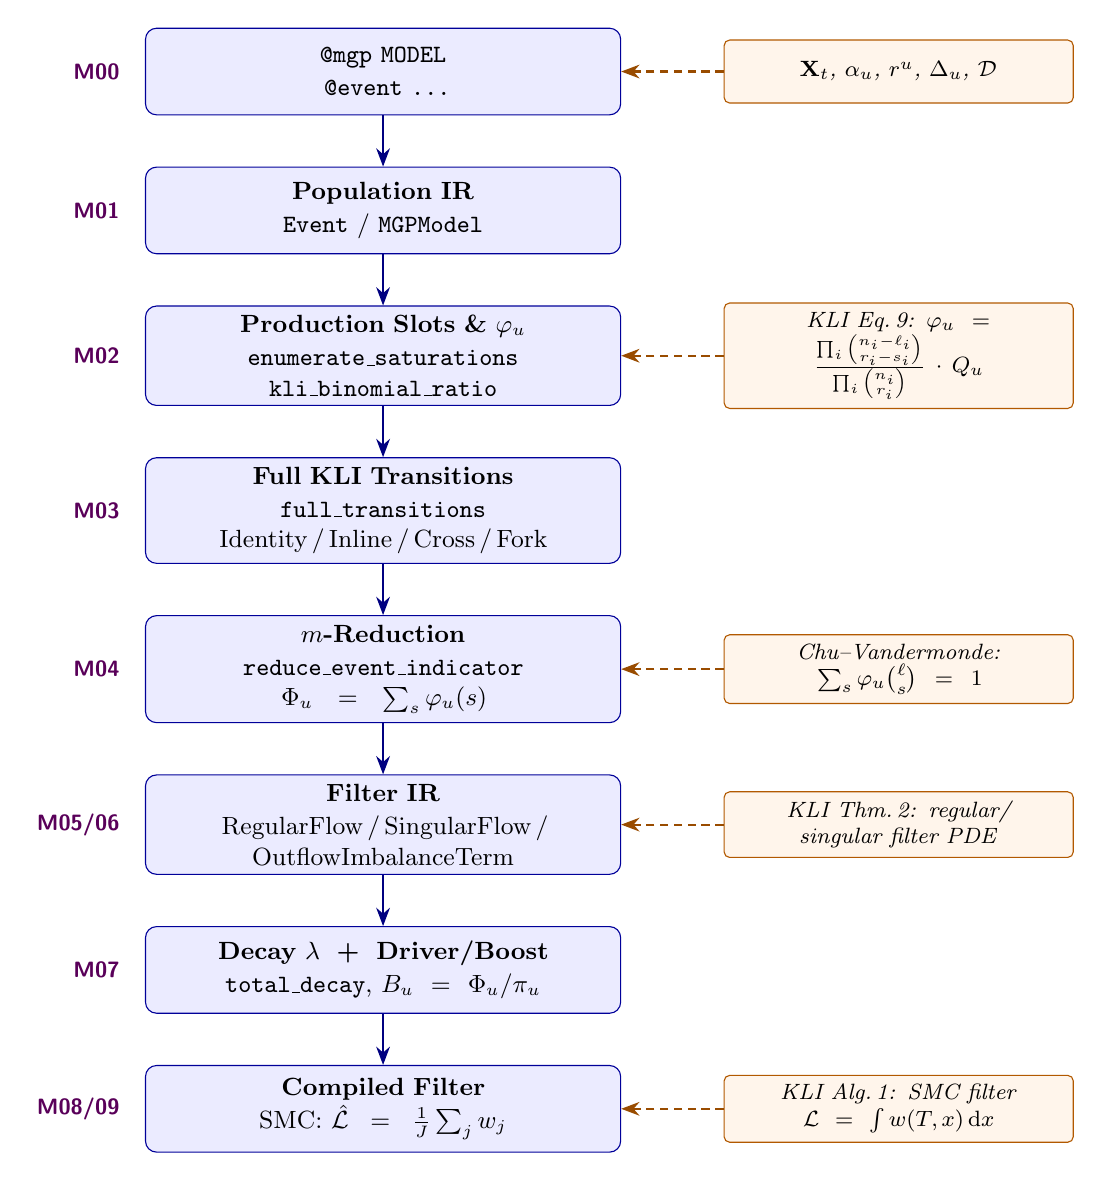
\begin{tikzpicture}[
    >=Stealth,
    stage/.style={
      rectangle, rounded corners=4pt,
      draw=blue!60!black, fill=blue!8,
      text width=5.8cm, minimum height=1.1cm,
      align=center, font=\small
    },
    klibox/.style={
      rectangle, rounded corners=2pt,
      draw=orange!70!black, fill=orange!8,
      text width=4.2cm, minimum height=0.8cm,
      align=center, font=\footnotesize\itshape
    },
    milestone/.style={
      font=\footnotesize\bfseries\sffamily, text=violet!70!black
    },
    arr/.style={->, thick, blue!50!black},
    karr/.style={->, densely dashed, orange!60!black, thick}
  ]

  % Pipeline stages
  \node[stage] (dsl)
    {\code{@mgp MODEL}\\[1pt]\code{@event ...}};
  \node[stage, below=0.65cm of dsl] (pir)
    {\textbf{Population IR}\\[1pt]
     \code{Event} / \code{MGPModel}};
  \node[stage, below=0.65cm of pir] (phi)
    {\textbf{Production Slots \& $\varphi_u$}\\[1pt]
     \code{enumerate\_saturations}\\
     \code{kli\_binomial\_ratio}};
  \node[stage, below=0.65cm of phi] (trans)
    {\textbf{Full KLI Transitions}\\[1pt]
     \code{full\_transitions}\\
     Identity\,/\,Inline\,/\,Cross\,/\,Fork};
  \node[stage, below=0.65cm of trans] (reduce)
    {\textbf{$m$-Reduction}\\[1pt]
     \code{reduce\_event\_indicator}\\
     $\Phi_u = \textstyle\sum_s \varphi_u(s)$};
  \node[stage, below=0.65cm of reduce] (fir)
    {\textbf{Filter IR}\\[1pt]
     RegularFlow\,/\,SingularFlow\,/\\
     OutflowImbalanceTerm};
  \node[stage, below=0.65cm of fir] (dbd)
    {\textbf{Decay $\lambda$ \;+\; Driver/Boost}\\[1pt]
     \code{total\_decay}, $B_u = \Phi_u/\pi_u$};
  \node[stage, below=0.65cm of dbd] (filter)
    {\textbf{Compiled Filter}\\[1pt]
     SMC: $\hat{\lik} = \frac{1}{J}\sum_j w_j$};

  % Arrows
  \draw[arr] (dsl) -- (pir);
  \draw[arr] (pir) -- (phi);
  \draw[arr] (phi) -- (trans);
  \draw[arr] (trans) -- (reduce);
  \draw[arr] (reduce) -- (fir);
  \draw[arr] (fir) -- (dbd);
  \draw[arr] (dbd) -- (filter);

  % KLI annotations
  \node[klibox, right=1.3cm of dsl] (k1)
    {$\Xr_t$, $\alpha_u$, $r^u$, $\Delta_u$, $\Demes$};
  \node[klibox, right=1.3cm of phi] (k2)
    {KLI Eq.\,9: $\varphi_u = \frac{\prod_i \binom{n_i-\ell_i}{r_i-s_i}}
      {\prod_i \binom{n_i}{r_i}} \cdot Q_u$};
  \node[klibox, right=1.3cm of reduce] (k4)
    {Chu--Vandermonde:\\
     $\sum_s \varphi_u \binom{\ell}{s} = 1$};
  \node[klibox, right=1.3cm of fir] (k5)
    {KLI Thm.\,2: regular/\\singular filter PDE};
  \node[klibox, right=1.3cm of filter] (k7)
    {KLI Alg.\,1: SMC filter\\
     $\lik = \int w(T,x)\dd{x}$};

  \draw[karr] (k1) -- (dsl);
  \draw[karr] (k2) -- (phi);
  \draw[karr] (k4) -- (reduce);
  \draw[karr] (k5) -- (fir);
  \draw[karr] (k7) -- (filter);

  % Milestone labels
  \node[milestone, left=0.2cm of dsl.west] {M00};
  \node[milestone, left=0.2cm of pir.west] {M01};
  \node[milestone, left=0.2cm of phi.west] {M02};
  \node[milestone, left=0.2cm of trans.west] {M03};
  \node[milestone, left=0.2cm of reduce.west] {M04};
  \node[milestone, left=0.2cm of fir.west] {M05/06};
  \node[milestone, left=0.2cm of dbd.west] {M07};
  \node[milestone, left=0.2cm of filter.west] {M08/09};
\end{tikzpicture}
\caption{The PhyloPOMP.jl compiler pipeline.  Each stage (blue boxes, left)
corresponds to a milestone and implements a specific KLI mathematical object
(orange boxes, right).  Arrows show data flow; dashed arrows show the KLI
equation each stage realizes.}
\label{fig:pipeline}
\end{figure}

The stages are not merely conceptually separate: each is a distinct source
file exporting ordinary callable functions, and each consumes only the
previous stage's output type.  Stage~2 reads nothing but the production
vector $r^u$ stored in the Population~IR; Stage~3 consumes Stage~2's
saturations and $\varphi_u$ values without re-deriving either; Stage~4
consumes Stage~3's transition vector; Stage~5 consumes Stage~4's reduced
transitions.  Because the interfaces are values rather than call-backs, every
stage is separately testable against a hand-derived oracle, which is what
makes the verification argument of Section~\ref{sec:non-circularity} possible at
all.

\paragraph{Reading the code excerpts.}
Each stage below carries a literal excerpt of the Julia source that implements
it, cited by file and line number.  One systematic substitution is applied
throughout: the sources use Unicode identifiers---$\varphi$, $\ell$, $\Phi$,
$\alpha$, $\theta$, $\Delta$, $\pi$, and Greek parameter names such as
$\beta$, $\sigma$, $\gamma$, $\omega$, $\psi$---which are transliterated to
their ASCII spellings (\code{phi}, \code{ell}, \code{Phi}, \code{alpha},
\code{theta}, \code{Delta}, \code{pi}, \code{beta}, \code{sigma}, \ldots) so
that they typeset inside \code{verbatim}.  A line consisting only of
\code{[...]} marks elided guard or comment code; the elided range is always
stated in the surrounding prose.  Everything else is the file's own text at
the cited lines.

\subsection{Stage 1: Model Declaration and Population IR (M00--M01)}

The user declares a population model using Julia macros.  The shipped SEIR
declaration is \code{mgp\_macro.jl:188--198}:
\begin{quote}
{\footnotesize
\begin{verbatim}
@mgp SEIR begin
    compartments = (S, E, I, R)
    demes = (E, I)
    params = (beta, sigma, gamma, omega, psi, chi, N)

    @event infection   rate=beta*S*I/N pop=(S=-1, E=+1) move=fork(I => E, I) kind=regular
    @event progression rate=sigma*E     pop=(E=-1, I=+1) move=swap(E => I)    kind=regular
    @event recovery    rate=gamma*I     pop=(I=-1, R=+1) move=chop(I)         kind=regular
    @event waning      rate=omega*R     pop=(R=-1, S=+1) move=none            kind=regular
    @event sampling    rate=psi*I     pop=()           move=sample(I)      kind=singular
end
\end{verbatim}
}
\end{quote}

In KLI terms, this declares:
\begin{itemize}
  \item The \textbf{deme set} $\Demes = \{\deme{E}, \deme{I}\}$, the
    compartments $(S,E,I,R)$, and the parameter names.  The macro requires
    all three declarations---\code{mgp\_macro.jl:169--171} errors if any of
    \code{compartments}, \code{demes}, or \code{params} is absent---and
    \code{mgp\_macro.jl:176} additionally requires $\Demes$ to be a
    \emph{subset} of the compartments, enforcing KLI's convention that a
    deme is a lineage-carrying compartment rather than a separate object.
  \item The \textbf{jump marks} $\Jumps =
    \{\text{infection}, \text{progression}, \text{recovery},
    \text{waning}, \text{sampling}\}$.
  \item For each mark $u \in \Jumps$:
    the \textbf{hazard function} $\alpha_u(t,x,x')$
    (from \code{rate=}),
    the \textbf{state-change vector} $\Delta_u$
    (from \code{pop=}),
    the \textbf{production vector} $r^u \in \Zp^{|\Demes|}$
    (inferred from \code{move=}),
    the \textbf{event type} (Birth/Death/Migration/Sample/Neutral),
    and whether the event is \textbf{regular} ($t \notin \mathrm{event}(\Pr)$)
    or \textbf{singular} ($t \in \mathrm{event}(\Pr)$).
\end{itemize}

% --- DSL-to-IR concrete mapping figure ---
\begin{figure}[ht]
\centering
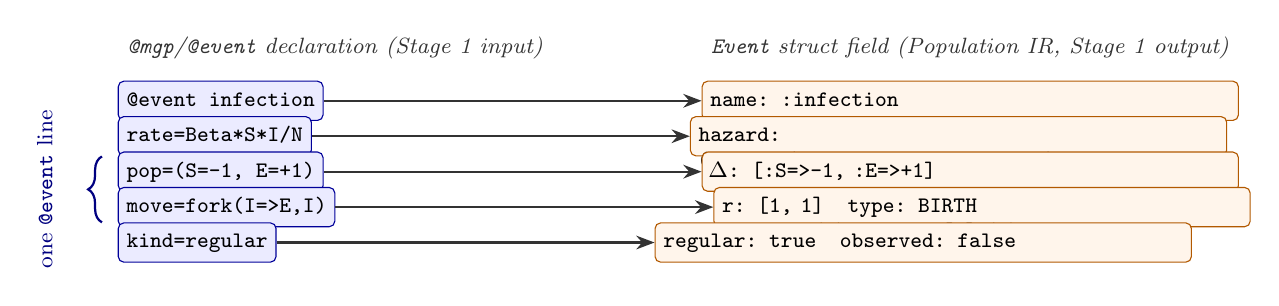
\begin{tikzpicture}[
    >=Stealth,
    dsltok/.style={
      rectangle, draw=blue!60!black, fill=blue!8, rounded corners=2pt,
      font=\ttfamily\footnotesize, inner sep=3pt, text height=1.4ex, text depth=0.5ex
    },
    irtok/.style={
      rectangle, draw=orange!70!black, fill=orange!8, rounded corners=2pt,
      font=\ttfamily\footnotesize, inner sep=3pt, text height=1.4ex, text depth=0.5ex,
      text width=6.6cm, align=left
    },
    lbl/.style={font=\footnotesize\itshape, text=gray!40!black},
    arr/.style={->, thick, gray!40!black}
  ]
  \node[dsltok] (d0) {@event infection};
  \node[dsltok, below=0.45cm of d0.west, anchor=west] (d1) {rate=Beta*S*I/N};
  \node[dsltok, below=0.45cm of d1.west, anchor=west] (d2) {pop=(S=-1, E=+1)};
  \node[dsltok, below=0.45cm of d2.west, anchor=west] (d3) {move=fork(I=>E,I)};
  \node[dsltok, below=0.45cm of d3.west, anchor=west] (d4) ;

  \node[irtok, right=4.8cm of d0] (i0) {\code{name}: \texttt{:infection}};
  \node[irtok, right=4.8cm of d1] (i1) {\code{hazard}: \texttt{(x,theta)->theta.Beta*x.S*x.I/theta.N}};
  \node[irtok, right=4.8cm of d2] (i2) {\code{$\Delta$}: \texttt{[:S=>-1, :E=>+1]}};
  \node[irtok, right=4.8cm of d3] (i3) {\code{r}: \texttt{[1, 1]}\quad \code{type}: \texttt{BIRTH}\\
                                          \code{from}: \texttt{2 (I)}\quad \code{into}: \texttt{[1] (E)}};
  \node[irtok, right=4.8cm of d4] (i4) {\code{regular}: \texttt{true}\quad \code{observed}: \texttt{false}};

  \draw[arr] (d0.east) -- (i0.west);
  \draw[arr] (d1.east) -- (i1.west);
  \draw[arr] (d2.east) -- (i2.west);
  \draw[arr] (d3.east) -- (i3.west);
  \draw[arr] (d4.east) -- (i4.west);

  \node[lbl, above=0.15cm of d0.north west, anchor=south west]
    {\code{@mgp}/\code{@event} declaration (Stage 1 input)};
  \node[lbl, above=0.15cm of i0.north west, anchor=south west]
    {\code{Event} struct field (Population IR, Stage 1 output)};

  \draw[decorate, decoration={brace, amplitude=5pt, mirror}, thick, blue!50!black]
    ([xshift=-0.2cm]d1.south west) -- ([xshift=-0.2cm]d4.north west)
    node[midway, left=0.5cm, font=\footnotesize, text=blue!50!black, align=right,
         rotate=90, anchor=south]
    {one \code{@event} line};
\end{tikzpicture}
\caption{Stage 1's lowering step, made concrete: SEIR's \code{infection}
mark, as written in the DSL (left, blue), and the fields of the
\code{Event} struct it is parsed into (right, orange) --- the Population
IR the rest of the compiler pipeline consumes. \code{mgp\_macro.jl}'s job
is exactly this rewrite: bare model symbols (\code{S}, \code{I},
\code{Beta}) in \code{rate=} become field accesses on the state/parameter
NamedTuples (\code{x.S}, \code{x.I}, \code{theta.Beta}), and the
declarative \code{move=fork(I=>E,I)} notation is decoded into the numeric
production vector~$r^u$, event type, and from/into deme indices.}
\label{fig:dsl-to-ir}
\end{figure}

The macro's only semantic act is a symbol rewrite: \code{\_rewrite}
(\code{mgp\_macro.jl:9--18}) walks the \code{rate=} expression tree and
replaces a bare compartment symbol by a field access on the state tuple and a
bare parameter symbol by a field access on the parameter tuple, so
\code{rate=beta*S*I/N} becomes the closure \code{(x,theta) ->
theta.beta*x.S*x.I/theta.N}.  No likelihood quantity is generated at
macro-expansion time; the macro emits data only.

Each declaration lowers into one \code{Event} struct, and the vector of them
into an \code{MGPModel}---the \emph{Population IR}.  These two structs are the
entire interface between the modelling language and every downstream stage
(\code{mgp.jl:59--69} and \code{mgp.jl:77--82}):
\begin{quote}
{\small
\begin{verbatim}
struct Event
    name     :: Symbol
    Delta    :: Vector{Pair{Symbol,Int}}
    hazard   :: Function
    r        :: Vector{Int}
    type     :: EventType
    from     :: Int
    into     :: Vector{Int}
    regular  :: Bool
    observed :: Bool
end
\end{verbatim}
}
\end{quote}
Field-by-field this is KLI's per-mark data: \code{hazard} is $\alpha_u$,
\code{Delta} is $\Delta_u$, \code{r} is the production vector $r^u$ indexed by
deme, \code{type} is one of the five pure event types of KLI \S3.2 (the
\code{@enum} at \code{mgp.jl:32}), \code{from} is the ancestral/source deme
$d_u$, \code{into} the target demes, and \code{regular} the
regular/singular flag.  Note what is \emph{absent}: neither the saturation
$s$ nor the lineage count $\ell$ is a field, because both depend on the
pruned genealogy at time $t$ and are therefore arguments supplied by the
filter at each event, not model data (\code{mgp.jl:52--57}).

The production vector is \emph{derived from the coloring operator}, not
declared.  \code{\_production} (\code{mgp\_macro.jl:61--67}) counts emergent
slots per deme, and the \code{:fork} branch of \code{\_decode\_move}
(\code{mgp\_macro.jl:78--86}) supplies the target list:
\begin{quote}
{\small
\begin{verbatim}
function _production(targets, demes)
    r = zeros(Int, length(demes))
    for target in targets
        r[_deme_index(target, demes)] += 1
    end
    r
end
[...]
    if op === :fork
        source, first_target = _arrow(ex.args[2])
        targets = _targets(first_target, ex.args[3:end])
        from = _deme_index(source, demes)
        into_demes = copy(targets)
        parent = findfirst(==(source), into_demes)
        isnothing(parent) || deleteat!(into_demes, parent)
        into = unique(_deme_index(d, demes) for d in into_demes)
        return BIRTH, from, collect(into), _production(targets, demes)
\end{verbatim}
}
\end{quote}
The \code{+=} at \code{mgp\_macro.jl:64} is what makes $r^u$ a multiset count
rather than a set: \code{move=fork(I => E, I)} has target list
$(\deme{E},\deme{I})$ and therefore $r^{\text{infection}} = (1,1)$---one slot
for the new exposed child and one for the still-infectious parent.  Lines
82--84 then delete the parent from \code{into} while leaving it in
\code{targets}, so \code{into} names the genuinely \emph{new} demes while $r^u$
counts \emph{every} emergent slot, the parent's included.  This distinction is
exactly what later gives \code{infection} a nonzero saturation component in
its own ancestral deme, hence the InlineSameDeme class of Stage~3.  The other
operators fall out the same way: \code{swap(E => I)} gives
$r^{\text{progression}} = (0,1)$ (\code{mgp\_macro.jl:87--93}),
\code{chop(I)} gives $r^{\text{recovery}} = (0,0)$ with no targets at all
(lines 94--96), and \code{sample(I)} gives $r^{\text{sampling}} = (0,1)$
(lines 97--100) because a non-destructive sample inserts a leaf slot on a
lineage that survives.

Milestone~M01 added \code{audit\_model} (\code{mgp\_audit.jl:97--111}) and
\code{validate\_model} (\code{mgp\_audit.jl:172}) that walk this IR,
confirming every $\Delta_u$, $\alpha_u$, $r^u$, and from/into wiring is
present and well-typed.  These duplicate, deliberately, checks the macro
already performs at expansion time---the point being that a hand-written
\code{MGPModel} such as \code{SEIR\_REFERENCE} (\code{mgp.jl:91--107}), which
never passes through \code{@mgp}, can be validated by the same code path.

\begin{remark}[Design decision]
A single \code{Event} struct with an \code{EventType} enum was retained
(not a typed subtype hierarchy), because the closed set of 4~stub functions
that dispatch on event semantics is small enough for \code{if}/\code{elseif}
branching.
\end{remark}

\subsection{Stage 2: Production Slots and the Binomial Ratio $\varphi_u$ (M02)}

Given an event with production $r^u$ and a lineage-count state~$\ell$,
the \textbf{saturation space} is:
\begin{equation}\label{eq:sat-space}
  S_u(\ell) = \bigl\{ s \in \Zp^{|\Demes|}
    : 0 \le s_i \le \min(r^u_i, \ell_i) \;\forall\, i \in \Demes \bigr\}.
\end{equation}
Each saturation $s$ specifies how many of the event's $r^u_i$ emergent
lineages in deme~$i$ are ``filled'' by tracked (pruned-tree) lineages.

\code{enumerate\_saturations} realizes~(\ref{eq:sat-space}) as a literal
Cartesian product (\code{mgp\_phi.jl:78--80}):
\begin{quote}
{\small
\begin{verbatim}
    D = length(r)
    ranges = ntuple(d -> 0:min(r[d], ell[d]), D)
    return [collect(Int, s) for s in vec(collect(Iterators.product(ranges...)))]
\end{verbatim}
}
\end{quote}
The \code{ntuple} on line~79 builds one range $0:\min(r^u_d,\ell_d)$ per deme,
which is exactly the per-coordinate constraint of~(\ref{eq:sat-space}), and
\code{Iterators.product} on line~80 forms their Cartesian product, so
$|S_u(\ell)| = \prod_{i}(\min(r^u_i,\ell_i)+1)$.  The two boundary cases KLI's
combinatorics require are consequences of the \code{min}, not special cases:
$\ell_d = 0$ collapses deme~$d$'s range to $\{0\}$ (a deme with no tracked
lineages cannot fill a slot), and $r^u_d = 0$ does likewise (nothing is
produced there, so nothing can be saturated there).

For each $s$, the \textbf{binomial ratio} (KLI Eq.\,9) is:
\begin{equation}\label{eq:phi}
  \varphi_u(s) = Q_u \cdot
  \prod_{i \in \Demes}
    \frac{\binom{n_i - \ell_i}{r^u_i - s_i}}{\binom{n_i}{r^u_i}},
\end{equation}
where $n_i = n_i(x)$ is the post-event deme occupancy and
$Q_u \in \{0,1\}$ is the compatibility indicator.

The body of \code{kli\_binomial\_ratio} (\code{mgp\_phi.jl:175--185}) is
(\ref{eq:phi}) transcribed one factor at a time:
\begin{quote}
{\small
\begin{verbatim}
    any(sd < 0 for sd in s) && return zero(Rational{Int})
    phi = Rational{Int}(Q)
    for d in 1:D
        denom = safe_binomial(n[d], r[d])
        if denom == 0
            return zero(Rational{Int})
        end
        numer = safe_binomial(n[d] - ell[d], r[d] - s[d])
        phi *= numer // denom
    end
    return phi
\end{verbatim}
}
\end{quote}
The \code{for d in 1:D} loop at \code{mgp\_phi.jl:177--184} computes exactly
the product in~(\ref{eq:phi}), one factor per deme: line~182 is the numerator
$\binom{n_i-\ell_i}{r^u_i-s_i}$, line~178 the denominator
$\binom{n_i}{r^u_i}$.  The accumulator is \emph{seeded} with the
compatibility indicator at line~176, so $Q_u$ multiplies the product rather
than gating it afterwards, which is why $Q_u = 0$ yields an exact zero rather
than a rounded one.  The \code{//} on line~183 is Julia's exact rational
division, so the return value is a \code{Rational\{Int\}} and boundary values
$0$ and $1$ are exactly comparable in tests---no floating-point tolerance
appears anywhere in Stages 2--6.

The three degenerate cases are handled by three \emph{different} mechanisms,
which is worth separating.  $s_i < 0$ is an explicit pre-check (line~175),
because $r_i - s_i$ would otherwise exceed $r_i$ and produce a nonzero
binomial for a nonsensical negative-count saturation.  $s_i > r^u_i$ needs no
guard at all: it makes $r_i - s_i < 0$, and $\binom{a}{b} = 0$ for $b<0$
already.  $n_i < r^u_i$ is caught as a zero \emph{denominator} (lines
179--181) and returns $0$---the saturation is unreachable given $n$---rather
than raising \code{DivideError}.  All three route through
\code{safe\_binomial} (\code{mgp\_phi.jl:103--106}):
\begin{quote}
{\small
\begin{verbatim}
function safe_binomial(a::Integer, b::Integer)
    (a < 0 || b < 0 || b > a) && return 0
    return binomial(a, b)
end
\end{verbatim}
}
\end{quote}
This wrapper is not defensive boilerplate: Julia's \code{Base.binomial}
extends to negative upper arguments by Pascal's rule, so
\code{binomial(-1,1) == -1}---asserted at load time in
\code{mgp\_phi.jl:116}---which is the wrong convention for a combinatorial
count of slots.  \code{safe\_binomial} imposes the KLI convention
$\binom{a}{b}=0$ outside range on all three arguments.

\subsection{Stage 3: Full KLI Transition Classification (M03)}

Each saturation $s \in S_u(\ell)$ licenses a specific \emph{full coloring
transition} $Y \to Y'$ on the pruned genealogy.  The function
\code{full\_transitions} classifies each~$s$ generically from
$\mathrm{sum}(s)$ and a comparison of the occupied slot's deme against
\code{event.from} (the ancestral deme):

\begin{center}
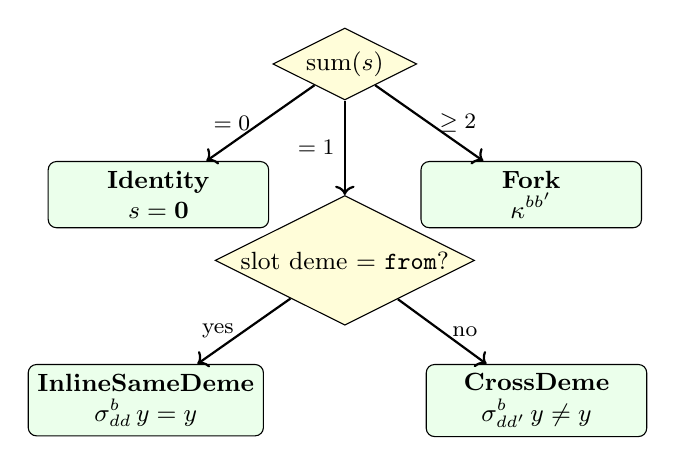
\begin{tikzpicture}[
    node distance=0.8cm and 1.5cm,
    box/.style={rectangle, rounded corners=3pt, draw, fill=green!8,
                minimum width=2.8cm, minimum height=0.7cm,
                align=center, font=\small},
    dec/.style={diamond, draw, fill=yellow!15, inner sep=1pt,
                font=\small, aspect=2},
    arr/.style={->, thick}
  ]
  \node[dec] (sum) {$\mathrm{sum}(s)$};
  \node[box, below left=1cm and 0.5cm of sum] (id)
    {\textbf{Identity}\\$s = \mathbf{0}$};
  \node[dec, below=1.2cm of sum] (one) {slot deme $=$ \code{from}?};
  \node[box, below left=0.9cm and 0.2cm of one] (inline)
    {\textbf{InlineSameDeme}\\$\sigma^b_{dd}\, y = y$};
  \node[box, below right=0.9cm and 0.2cm of one] (cross)
    {\textbf{CrossDeme}\\$\sigma^b_{d d'}\, y \ne y$};
  \node[box, below right=1cm and 0.5cm of sum] (fork)
    {\textbf{Fork}\\$\kappa^{bb'}$};

  \draw[arr] (sum) -- node[left,font=\footnotesize]{$=0$} (id);
  \draw[arr] (sum) -- node[left,font=\footnotesize]{$=1$} (one);
  \draw[arr] (sum) -- node[right,font=\footnotesize]{$\ge 2$} (fork);
  \draw[arr] (one) -- node[left,font=\footnotesize]{yes} (inline);
  \draw[arr] (one) -- node[right,font=\footnotesize]{no} (cross);
\end{tikzpicture}
\end{center}

The decision tree above is not a diagrammatic gloss---it is the literal
control flow of \code{mgp\_transitions.jl:230--250}:
\begin{quote}
{\small
\begin{verbatim}
    for (i, s) in enumerate(S)
        phi = kli_binomial_ratio(r, s, ell, n; Q = Q)
        total = sum(s)
        transitions[i] = if total == 0
            IdentityTransition(event, s, phi)
        elseif total == 1
            d = findfirst(!=(0), s)
            if d == ancestral
                InlineSameDemeTransition(event, s, phi, d)
            else
                CrossDemeTransition(event, s, phi, ancestral, d)
            end
        else
            slot_demes = Int[]
            for d in eachindex(s)
                for _ in 1:s[d]
                    push!(slot_demes, d)
                end
            end
            ForkTransition(event, s, phi, ancestral, slot_demes)
        end
    end
\end{verbatim}
}
\end{quote}
Line~232's \code{total = sum(s)} is the diagram's root test, and line~237's
\code{d == ancestral} is its second, where \code{ancestral = event.from} was
bound once at \code{mgp\_transitions.jl:226}.  Binding it \emph{once, outside
the loop} is the coded form of a mathematical claim: for a given mark, every
occupied slot has the same ancestral deme, namely the single source deme
$d_u$, whatever the slot's post-event deme happens to be---so the
InlineSameDeme/CrossDeme test is a comparison against a per-event constant,
not a per-slot lookup.  Note also that $\varphi_u$ is computed on line~231
for \emph{every} feasible $s$ regardless of class, so classification never
alters a weight; it only labels one.

The Fork branch (lines 243--248) expands $s$ into a \emph{multiset}
\code{slot\_demes} with one entry per occupied slot, repeated $s_d$ times.
That is what keeps $s=(2,0)$---a within-deme branch point, two slots in
deme~1---distinguishable from $s=(1,1)$, a cross-deme spillover branch point;
both have $\mathrm{sum}(s)=2$ and would be indistinguishable under a
set-valued representation.

Finally, \code{full\_transitions} accepts only \code{BIRTH} and
\code{MIGRATION} events and throws on the rest
(\code{mgp\_transitions.jl:212--219}).  This is a scope boundary drawn by
event \emph{type}, not by whether $r^u$ happens to vanish: KLI compatibility
for Death and Sample marks is rate-driven, and those marks are picked up
instead by the decay machinery of Stage~6.

\begin{remark}
\textbf{Identity} and \textbf{InlineSameDeme} are distinct at the full-KLI
level---they differ in the event-indicator component~$m$---even though both
leave the reduced coloring unchanged ($y' = y$ on the deme-only state).
This distinction is central to the correctness of $m$-marginalization
(Stage~4).
\end{remark}

\subsection{Stage 4: Reduction over the Event Indicator $m$ (M04)}

The coloring $Y_t(a) = (\mathrm{col}(Y), \mathrm{ctr}(Y))$ has a
\emph{color} (deme) component and an \emph{event indicator}
component~$m$.  KLI's filter equation acts on the reduced, color-only
state.  The function \code{reduce\_event\_indicator} groups the full
transitions by their outcome on the reduced \code{Coloring} and sums:
\begin{equation}\label{eq:Phi}
  \Phi_u(d, d') = \sum_{\substack{s \in S_u(\ell) \\
    \text{reducing to } d \to d'}} \varphi_u(s).
\end{equation}
(As in the rest of this report, $\Phi_u$ is our own name for this
$m$-marginalized sum; KLI performs the same sum but does not give it this
symbol.)

The collapsing rule is a four-line dispatch table
(\code{mgp\_reduce.jl:115--119}), traced to the actual \code{swap!} code in
\code{coloring.jl} rather than to the paper's informal notation:
\begin{quote}
{\small
\begin{verbatim}
reduced_key(t::IdentityTransition) = (:noop, t.event.from)
reduced_key(t::InlineSameDemeTransition) = (:noop, t.deme)
reduced_key(t::CrossDemeTransition) = (:cross, t.ancestral_deme, t.target_deme)
reduced_key(t::ForkTransition) =
    (:fork, t.ancestral_deme, Tuple(sort(t.slot_demes)))
\end{verbatim}
}
\end{quote}
Two full transitions collapse together precisely when these keys are equal,
so:
\begin{itemize}
  \item \textbf{Identity} $+$ \textbf{InlineSameDeme} $\to$ single
    \code{(:noop, d)} group.  Lines 115 and 116 return the same key because
    \code{t.event.from} and \code{t.deme} are the same deme index for an
    InlineSameDeme transition (that is what ``inline'' means, by Stage~3's
    line~237 test), and because \code{swap!(y,i,i,b)} is a literal no-op on
    the \code{BitSet}: a \code{delete!} followed by a \code{push!} of the same
    lineage id into the same deme's set.
  \item \textbf{CrossDeme} $\to$ its own \code{(:cross, d, d')} group
    (because \code{swap!(y,i,j,b)} with $i \ne j$ genuinely changes the
    coloring), one group per distinct ordered deme pair.
  \item \textbf{Fork} $\to$ its own \code{(:fork, d, \ldots)} group.
\end{itemize}
The fork key deserves a note.  Equation~(\ref{eq:Phi}) indexes $\Phi_u$ by an
ordered pair $(d,d')$, which is the right index for the \code{:noop} case
($d\to d$) and the \code{:cross} case; a branch point, however, is not a pair
but an ancestral deme together with a \emph{multiset} of post-event slot
demes, which is what line~119's \code{Tuple(sort(...))} produces.  Sorting
makes the key order-independent while \code{Tuple} preserves multiplicity, so
two genuinely different Fork saturations of the same event that happened to
land in the same demes \emph{would} correctly collapse.  No current
SEIR/MERS/SI2R event exercises that---each has at most one Fork-classified
saturation---but the key is generic rather than a special case of ``there is
only ever one fork'' (\code{mgp\_reduce.jl:45--56}).

The summation itself is \code{mgp\_reduce.jl:162--168}:
\begin{quote}
{\small
\begin{verbatim}
    result = Vector{ReducedTransition}(undef, length(order))
    for (i, k) in enumerate(order)
        members = groups[k]
        Phi = sum(t.phi for t in members)
        result[i] = ReducedTransition(k, reduced_kind(members[1]), Phi, members)
    end
    return result
\end{verbatim}
}
\end{quote}
Line~165 is (\ref{eq:Phi}): an exact \code{Rational\{Int\}} sum of the
$\varphi_u(s)$ over precisely those $s$ that share a reduced key.  Two
implementation choices carry mathematical weight.  First, the grouping is
driven by an insertion-ordered key vector (\code{order}, built at lines
152--161) rather than by dictionary iteration order, so the output sequence is
deterministic across runs---a prerequisite for the bit-for-bit RNG-order
comparisons of Stage~7.  Second, the contributing \code{members} are retained
in the result rather than discarded, so every $\Phi_u$ can be traced back to
the exact set of full transitions that produced it; the audit and explain
tooling of the later milestones reads that provenance.

The Chu--Vandermonde identity guarantees the partition-of-unity:
\begin{equation}\label{eq:cv}
  \sum_{s \in \Zp^{|\Demes|}}
  \varphi_u(s) \binom{\ell}{s} = 1,
\end{equation}
whenever $n_i \ge \{\ell_i, r^u_i\}$ for all $i$.  No compiler function
computes~(\ref{eq:cv}); it is an identity the compiler's output must satisfy,
and it is therefore checked in the test suite rather than implemented.  The
broadest such check assembles the sum directly from Stage~2's two functions
(\code{test/kli\_si2r\_test.jl:480--486}):
\begin{quote}
{\small
\begin{verbatim}
                sats = enumerate_saturations(ev.r, ell)
                cv_sum = Rational{Int}(0)
                for s in sats
                    phi = kli_binomial_ratio(ev, s, ell, n)
                    cv_sum += phi * prod(binomial(ell[d], s[d]) for d in 1:2)
                end
                @test cv_sum == 1 // 1
\end{verbatim}
}
\end{quote}
Line~484's \code{prod(binomial(ell[d], s[d]) ...)} is the multinomial weight
$\binom{\ell}{s}$ of~(\ref{eq:cv}), and line~486 asserts \emph{exact} equality
to $1$ in $\mathbb{Q}$---not equality within a tolerance.  This runs over 200
randomized $(\ell,n)$ states $\times$ 4 events.  A separate M12 property test
(\code{test/kli\_properties\_test.jl:115--131}, 500 randomized trials) checks
the weaker but structurally distinct conservation law $\sum_s \varphi_u(s) =
\sum_{\text{groups}} \Phi_u$: that Stage~4 partitions Stage~3's mass without
dropping or duplicating any of it.

\subsection{Stage 5: Filter IR Classification (M05/M06)}

Each \code{ReducedTransition} is classified as:
\begin{center}
\renewcommand{\arraystretch}{1.2}
\begin{tabular}{@{}p{0.24\textwidth}p{0.27\textwidth}p{0.36\textwidth}@{}}
\toprule
\textbf{Bucket} & \textbf{Condition} & \textbf{KLI role} \\
\midrule
\textbf{RegularFlow} & \code{:noop} or \code{:cross},
  \code{event.regular} &
  Inflow term: $\alpha_u \cdot \Phi_u$ (non-fork) \\
\textbf{SingularFlow} & any kind, \code{!event.regular} &
  Fixed observed-event-time contribution \\
\textbf{OutflowImbalanceTerm} & \code{:fork}, \code{event.regular} &
  Fork mass resolved by inflow/outflow balance \\
\bottomrule
\end{tabular}
\end{center}

The table is the function \code{classify\_filter\_terms}
(\code{mgp\_filter\_ir.jl:317--334}), row for row:
\begin{quote}
{\small
\begin{verbatim}
    if event.regular
        for rt in reduced
            if rt.kind == :noop || rt.kind == :cross
                push!(regular, RegularFlow(event, rt, rt.Phi))
            elseif rt.kind == :fork
                push!(outflow_imbalance,
                      OutflowImbalanceTerm(event, rt, rt.Phi, :inflow_outflow_imbalance,
                                            :fork_unobserved_at_regular_time))
            else
                throw(ArgumentError("classify_filter_terms: unrecognized " *
                                     "ReducedTransition.kind `$(rt.kind)`"))
            end
        end
    else
        for rt in reduced
            push!(singular, SingularFlow(event, rt, rt.Phi))
        end
    end
\end{verbatim}
}
\end{quote}
The classification reads only two bits of information---\code{event.regular}
(line~317) and \code{rt.kind} (lines 319, 321)---and nothing about any
proposal kernel.  That is deliberate: the Filter~IR describes the
\emph{target} filter structure, so it must be identical whichever of the
four proposal strategies of Stage~6 will later be used to sample it.  Note
too that $\Phi$ is copied verbatim from the \code{ReducedTransition}
(\code{rt.Phi} at lines 320, 323, 332) and never recomputed or rescaled; a
term's numeric content is entirely Stage~4's, and Stage~5 contributes only the
bucket label plus the \code{mechanism}/\code{reason} tags that record why.
Before classifying, the function checks that every full transition's
provenance actually names the \code{event} argument
(\code{mgp\_filter\_ir.jl:305--311}) and throws otherwise, so one event's
reduced transitions cannot be silently filed under another's.

Two limitations are recorded in the source rather than papered over.  The
\code{else} branch at lines 330--334 is unreachable for every shipped model:
no SEIR, MERS, or SI2R \code{BIRTH}/\code{MIGRATION} event has
\code{regular == false}, and the singular events that do exist are all
\code{SAMPLE}-typed and hence outside \code{full\_transitions}' scope
(\code{mgp\_filter\_ir.jl:291--297}), so \code{SingularFlow} is exercised only
against a synthetic hand-built \code{Event} in
\code{test/kli\_filter\_ir\_test.jl}.  And the \code{OutflowImbalanceTerm}
constructed at lines 322--324 carries only provenance: its $\Phi$ field is the
raw reduced sum, not a computed imbalance weight.

\begin{remark}[M06 correction]
M05's original name ``DecayTerm'' was renamed to
``\textbf{OutflowImbalanceTerm}'' because this bucket is \emph{not}
KLI's $\lambda(t,x,y)$---that is a separate mechanism (sampling hazard
$+$ sub-threshold removal).  The fork/branch-point mass is resolved by
the structural imbalance between the full-hazard regular outflow and
the non-fork-only inflow, per the KLI paper's explicit warning:
\emph{``Adding either to $\lambda$ would double-count.''}
The rename was made structural, not cosmetic: after M06 there is no type or
field anywhere in \code{mgp\_filter\_ir.jl} whose name contains ``decay'', and
the \code{mechanism} tag is fixed at \code{:inflow\_outflow\_imbalance}, so a
later implementer of $\lambda$ cannot reach for a plausible-looking
\code{FilterSpec.decay} field and sum it in---the field does not exist.
\end{remark}

\subsection{Stage 6: Decay $\lambda$ and Driver/Boost (M07)}

KLI's \textbf{decay term} is:
\begin{equation}\label{eq:decay}
  \lambda(t,x,y) = \underbrace{\sum_{u:\,\text{SAMPLE}}
    \alpha_u(x,\theta)}_{\text{sampling hazard}}
  + \underbrace{\sum_{u:\,\text{DEATH}}
    \alpha_u(x,\theta) \cdot \indicator{n_{d_u} \le \ell_{d_u}}}_{%
    \text{sub-threshold removal}},
\end{equation}
where $d_u = \text{event.from}$ is the deme the death event acts on.
The two summands of~(\ref{eq:decay}) are the two branches of
\code{decay\_contribution} (\code{mgp\_decay.jl:247--252} and
\code{262--270}, with the argument-validation guards at lines 253--261
elided):
\begin{quote}
{\small
\begin{verbatim}
    alpha = event.hazard(x, theta)

    if event.type == SAMPLE
        gate   = one(Rational{Int})
        reason = :sampling_hazard_full
    else # DEATH
        d = event.from
[...]
        elld, nd = ell[d], n[d]
[...]
        gate   = nd <= elld ? one(Rational{Int}) : zero(Rational{Int})
        reason = :sub_threshold_removal
    end

    DecayContribution(event, alpha, gate, alpha * gate, reason)
\end{verbatim}
}
\end{quote}
Line~250's unconditional \code{one(Rational\{Int\})} is the first summand's
missing indicator: a Sample mark contributes its \emph{full} hazard, because
the exact likelihood conditions on no sample having occurred at any
$t \notin \mathrm{event}(\Pr)$, and no threshold question arises.  Line~266's
ternary is the indicator $\indicator{n_{d_u} \le \ell_{d_u}}$ of the second
summand.  Two details are load-bearing.  First, \code{gate} is a
\code{Rational}, not a \code{Bool}, so line~270's \code{alpha * gate} stays in
exact arithmetic whenever the hazard itself is rational---which is how the
decay tests hand-verify values.  Second, the invariant $\ell_d \le n_d$ is
asserted (line~263, throwing if violated) rather than assumed, and under it
the condition $n_d \le \ell_d$ collapses to $n_d = \ell_d$ exactly: the decay
fires only at the boundary where a removal has no compatible untracked target
left (\code{mgp\_decay.jl:44--50}).

The model-level $\lambda$ is the sum over marks
(\code{mgp\_decay.jl:290--295}):
\begin{quote}
{\small
\begin{verbatim}
    total = zero(Rational{Int})
    for event in model.events
        event.type in (DEATH, SAMPLE) || continue
        total += decay_contribution(event, x, theta, ell, n).value
    end
    total
\end{verbatim}
}
\end{quote}
The \code{continue} on line~292 is the reason (\ref{eq:decay}) has exactly two
summands and no others: \code{BIRTH}/\code{MIGRATION} marks belong to the
Filter~IR of Stage~5, and \code{NEUTRAL} marks contribute nothing at all,
because a neutral mark never touches the coloring and so has no compatibility
condition that could fail (\code{mgp\_decay.jl:73--80}).  The loop is
generic over \code{model.events}, so a model with three sampling channels or
five removal channels needs no new code.

The \textbf{driver} and \textbf{boost} decompose the filter's inflow
term:
\begin{equation}\label{eq:driver-boost}
  \beta_u = \alpha_u \cdot \pi_u, \qquad
  B_u = \frac{\Phi_u}{\pi_u},
\end{equation}
where $\pi_u$ is the proposal kernel's probability of choosing the
reduced outcome.  Both are one-liners (\code{mgp\_proposal.jl:96} and
\code{mgp\_proposal.jl:123}, with the convenience overload at line~132):
\begin{quote}
{\small
\begin{verbatim}
driver(alpha::Real, pi::Real) = alpha * pi

boost(Phi::Rational{Int}, pi::Real) = Phi / pi

boost(rt::ReducedTransition, pi::Real) = boost(rt.Phi, pi)
\end{verbatim}
}
\end{quote}
These are trivial by design, and naming them is the point:
(\ref{eq:driver-boost}) was previously implicit inside eight separately
hand-coded kernels, and the composition $\beta_u B_u = \alpha_u \pi_u \cdot
(\Phi_u/\pi_u) = \alpha_u \Phi_u$ is what makes the proposal cancel out of the
filter's expectation, so every kernel---naive, soft, guided, or hard---must
satisfy it however $\pi_u$ itself is built.  The four strategies are
represented only as tags (\code{ProposalStrategy} and its subtypes,
\code{mgp\_proposal.jl:60--78}); $\pi_u$ is not derived generically anywhere
in the compiler, by an explicit M00 decision to keep the existing,
already-tested hand-designed kernels.

One subtlety in \code{boost} is easy to get wrong and is documented at
\code{mgp\_proposal.jl:108--116}: the $\pi$ passed in must be the
\emph{fully marginalized} probability of the reduced outcome, including any
within-outcome degrees of freedom the concrete kernel introduces---for the
naive SEIR kernel, the top-level categorical probability of the mark
\emph{times} the uniform $1/\ell$ choice of which tracked lineage it acts
on---and not merely the top-level entry that a hand-coded kernel happens to
store in a variable named \code{pi}.  Using the unmarginalized value would
leave $\beta_u B_u \ne \alpha_u \Phi_u$ by exactly the lineage-choice factor.

\subsection{Stage 7: Compiled End-to-End Filters (M08/M09)}

Milestones M08 and M09 assembled the M01--M07 building blocks into
executable, model-specific compiled filters for SEIR and MERS,
respectively.  Each compiled filter is a structural mirror of the
corresponding hand-coded reference filter (\code{seir\_naive.jl},
\code{mers\_naive.jl})---identical control flow and RNG-call order, but
every likelihood term sourced from the generic compiler IR rather than
hand-derived closed forms.

The mirroring is literal.  Inside
\code{compiled\_regular\_part!} (\code{mgp\_seir\_filter.jl:232}), the two
infection branches call back into Stage~3 at run time
(\code{mgp\_seir\_filter.jl:276--277} and \code{286}, and \code{300--302};
the intervening lines 278--285 are an explanatory comment):
\begin{quote}
{\small
\begin{verbatim}
                    ts = full_transitions(infection, ellpost, npost)
                    Phiid = only(filter(t -> t isa IdentityTransition, ts)).phi
[...]
                    ll += log(Float64(Phiid)) - log(pi_[1])
\end{verbatim}
}
\end{quote}
\begin{quote}
{\small
\begin{verbatim}
                    ts = full_transitions(infection, ellpost, npost)
                    Phicr = only(filter(t -> t isa CrossDemeTransition, ts)).phi
                    ll += log(Float64(Phicr)) - log(1 / ellI_pre)
\end{verbatim}
}
\end{quote}
Lines 286 and 302 are $\log B_u$ of~(\ref{eq:driver-boost}) written out:
$\log \Phi_u - \log \pi_u$, with $\pi_u$ the naive kernel's
\code{pi\_[1]} in the no-op branch and its marginalized lineage-choice
probability $1/\ell_{\deme{I}}$ in the cross-deme branch.  The
\code{only(filter(...))} selects a \emph{single} full transition class rather
than the \code{:noop} reduced group, and the reason is a $Q_u$ fact:
the naive regular proposal never realizes the InlineSameDeme saturation, so
adding its mass---as \code{reduce\_event\_indicator} would---would
double-count probability the proposal structurally never proposes.  This is
the one place where regular-versus-singular $Q_u$ gating, deferred through
M03--M06, is actually applied.

The decay used by the compiled filter is $\lambda$ \emph{plus} a
proposal-specific correction (\code{mgp\_seir\_filter.jl:136--147}):
\begin{quote}
{\small
\begin{verbatim}
    total = Float64(total_decay(model, x, theta, ell, n))
    for event in model.events
        event.type == DEATH || continue
        d = event.from
        alphafull = Float64(event.hazard(x, theta))
        nd, elld = n[d], ell[d]
        above = nd > elld
        alphareduced = above ? alphafull * (nd - elld) / nd : 0.0
        leftover = (above ? alphafull : 0.0) - alphareduced
        total += leftover
    end
\end{verbatim}
}
\end{quote}
Line~136 is exactly (\ref{eq:decay}); lines 137--146 add, per Death mark, the
difference between the full hazard and the $\ell$-reduced hazard actually
offered to the regular proposal.  This term is not part of~(\ref{eq:decay})
and is not claimed to be: it is bookkeeping specific to a single-particle
importance sampler, which has no neighbouring population state to cancel the
``a tracked lineage died unobserved'' mass against.  The source flags its own
justification as ``a plausible, internally-consistent reading, not a proven
one'' (\code{mgp\_decay.jl:171--174}), with Gate~5 below as the empirical
check.

\begin{figure}[ht]
\centering
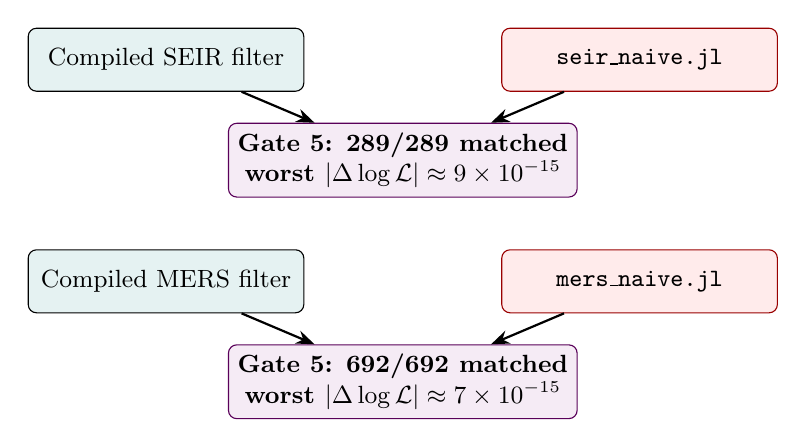
\begin{tikzpicture}[
    >=Stealth,
    box/.style={rectangle, rounded corners=3pt, draw, fill=teal!10,
                minimum width=3.5cm, minimum height=0.8cm,
                align=center, font=\small},
    ref/.style={rectangle, rounded corners=3pt, draw=red!60!black,
                fill=red!8,
                minimum width=3.5cm, minimum height=0.8cm,
                align=center, font=\small},
    gate/.style={rectangle, rounded corners=3pt, draw=violet!70!black,
                 fill=violet!8, minimum width=3.5cm, minimum height=0.8cm,
                 align=center, font=\small\bfseries},
    arr/.style={->, thick}
  ]
  \node[box] (cseir) {Compiled SEIR filter};
  \node[ref, right=2.5cm of cseir] (nseir) {\code{seir\_naive.jl}};
  \node[gate, below=0.8cm of $(cseir)!0.5!(nseir)$] (g5seir)
    {Gate 5: 289/289 matched\\worst $|\Delta\log\lik| \approx 9\times 10^{-15}$};
  \draw[arr] (cseir) -- (g5seir);
  \draw[arr] (nseir) -- (g5seir);

  \node[box, below=2cm of cseir] (cmers) {Compiled MERS filter};
  \node[ref, right=2.5cm of cmers] (nmers) {\code{mers\_naive.jl}};
  \node[gate, below=0.8cm of $(cmers)!0.5!(nmers)$] (g5mers)
    {Gate 5: 692/692 matched\\worst $|\Delta\log\lik| \approx 7\times 10^{-15}$};
  \draw[arr] (cmers) -- (g5mers);
  \draw[arr] (nmers) -- (g5mers);
\end{tikzpicture}
\caption{Gate~5 (numerical equivalence) validation.  Compiled filters and
hand-coded reference filters are run with identical seeds ($N_p = 1$), and
their log-likelihoods are compared.  All finite comparisons match to
floating-point noise.}
\label{fig:gate5}
\end{figure}

The $10^{-15}$ residuals of Figure~\ref{fig:gate5} are the signature of the
design: because Stages 2--6 work in exact $\mathbb{Q}$ and only the final
\code{log(Float64(...))} conversions introduce rounding, the compiled and
hand-coded filters agree to within a few units in the last place of a
\code{Float64}, not to within a tuned tolerance.  Anything larger would
indicate an algebraic disagreement rather than an arithmetic one.

\subsection{Code \texorpdfstring{$\leftrightarrow$}{<->} Math Correspondence}

Table~\ref{tab:correspondence} indexes every KLI object named in this section
against the equation that defines it here and the Julia code that computes it.
Line numbers refer to the files as read at the time of writing; each cited
range is the body of the computation, not the surrounding docstring.

\footnotesize
\renewcommand{\arraystretch}{1.15}
\begin{longtable}{@{}p{0.24\textwidth}p{0.07\textwidth}p{0.20\textwidth}p{0.30\textwidth}@{}}
\caption{Correspondence between the KLI objects of this section, the
equations that define them, and the Julia code that computes them.  Entries
with ``---'' in the equation column are structural rather than numerical:
they build or validate the intermediate representation that the numbered
equations are then evaluated against.}
\label{tab:correspondence}\\
\toprule
\textbf{KLI object} & \textbf{Equation} & \textbf{Julia function} &
  \textbf{file:line} \\
\midrule
\endfirsthead
\multicolumn{4}{l}{\textit{Table~\ref{tab:correspondence} continued from previous page}}\\
\toprule
\textbf{KLI object} & \textbf{Equation} & \textbf{Julia function} &
  \textbf{file:line} \\
\midrule
\endhead
\midrule
\multicolumn{4}{r}{\textit{continued on next page}}\\
\endfoot
\bottomrule
\endlastfoot
Population process data $(\alpha_u,\Delta_u,r^u)$ & --- &
  \code{Event}, \code{MGPModel} & \code{mgp.jl:59--82} \\
Deme set $\Demes$, marks $\Jumps$ & --- &
  \code{@mgp}, \code{@event} & \code{mgp\_macro.jl:149--186} \\
Hazard closure $\alpha_u(t,x)$ & --- &
  \code{\_rewrite} & \code{mgp\_macro.jl:9--18} \\
Production vector $r^u$ & --- &
  \code{\_production}, \code{\_decode\_move} & \code{mgp\_macro.jl:61--67, 69--106} \\
IR well-formedness & --- &
  \code{audit\_model}, \code{validate\_model} & \code{mgp\_audit.jl:97--111, 172} \\
\addlinespace
Saturation space $S_u(\ell)$ & \eqref{eq:sat-space} &
  \code{enumerate\_saturations} & \code{mgp\_phi.jl:73--81} \\
Binomial ratio $\varphi_u(s)$ & \eqref{eq:phi} &
  \code{kli\_binomial\_ratio} & \code{mgp\_phi.jl:167--186} \\
Convention $\binom{a}{b}=0$ off-range & \eqref{eq:phi} &
  \code{safe\_binomial} & \code{mgp\_phi.jl:103--106} \\
\addlinespace
Coloring transitions $\chi,\sigma,\kappa$ & --- &
  \code{full\_transitions} & \code{mgp\_transitions.jl:210--253} \\
Class of a saturation & --- &
  classification branch & \code{mgp\_transitions.jl:230--250} \\
\addlinespace
Reduction over $m$ (grouping key) & \eqref{eq:Phi} &
  \code{reduced\_key} & \code{mgp\_reduce.jl:115--119} \\
Reduced factor $\Phi_u$ & \eqref{eq:Phi} &
  \code{reduce\_event\_indicator} & \code{mgp\_reduce.jl:151--169} \\
Chu--Vandermonde check & \eqref{eq:cv} &
  (identity; no compiler function) & \code{test/kli\_si2r\_test.jl:480--486} \\
Full-to-reduced conservation & \eqref{eq:Phi} &
  (M12 property P2) & \code{test/kli\_properties\_test.jl:115--131} \\
\addlinespace
Filter IR buckets & --- &
  \code{classify\_filter\_terms} & \code{mgp\_filter\_ir.jl:304--337} \\
Regular / singular / fork terms & --- &
  \code{RegularFlow}, \code{SingularFlow}, & \code{mgp\_filter\_ir.jl:153--157,} \\
 & & \code{OutflowImbalanceTerm} & \code{183--187, 241--247} \\
\addlinespace
Per-mark decay & \eqref{eq:decay} &
  \code{decay\_contribution} & \code{mgp\_decay.jl:237--271} \\
Decay $\lambda(t,x,y)$ & \eqref{eq:decay} &
  \code{total\_decay} & \code{mgp\_decay.jl:287--296} \\
Driver $\beta_u = \alpha_u\pi_u$ & \eqref{eq:driver-boost} &
  \code{driver} & \code{mgp\_proposal.jl:96} \\
Boost $B_u = \Phi_u/\pi_u$ & \eqref{eq:driver-boost} &
  \code{boost} & \code{mgp\_proposal.jl:123, 132} \\
Proposal families $\pi_u$ & --- &
  \code{ProposalStrategy} subtypes & \code{mgp\_proposal.jl:60--78} \\
\addlinespace
Compiled decay (SEIR) & \eqref{eq:decay} &
  \code{compiled\_decay} & \code{mgp\_seir\_filter.jl:133--148} \\
Compiled boost at run time & \eqref{eq:driver-boost} &
  \code{compiled\_regular\_part!} & \code{mgp\_seir\_filter.jl:232--302} \\
Compiled likelihood $\lik$ & \eqref{eq:phylo-lik} &
  \code{compiled\_filter\_pomp} & \code{mgp\_seir\_filter.jl:357} \\
Compiled MERS filter & \eqref{eq:phylo-lik} &
  \code{mers\_compiled\_regular\_part!} & \code{mgp\_mers\_filter.jl:304} \\
\end{longtable}

Read down the table, the pipeline's shape is visible in the file column
alone: one file per stage, each depending only on the one above it, and the
two \code{test/} rows sitting where a mathematical identity---not a
computation---is what has to hold.


% ============================================================================
\section{The Mathematics}
\label{sec:math}
% ============================================================================

This section states, in KLI's own terms, the mathematical objects that the
compiler manipulates.  Every definition below is quoted or transcribed from
the reference text, and each is tagged with the section or equation number of
that text in which it appears, so that a reader can check the correspondence
directly.  Where this report uses notation that is \emph{not} KLI's, that is
flagged explicitly---see Remark~\ref{rem:phi-provenance} and
Table~\ref{tab:notation}.

\subsection{From population process to filter equation}

\subsubsection{The population process $\Xr_t$}

Let $\Xr_t$ be a continuous-time Markov process on the state
space~$\Xspace$ with initial density~$p_0$.  Following KLI~\S2.5
(``Jump marks''), the jumps of $\Xr_t$ are divided into categories
``which differ with respect to the changes they induce in a
genealogy'': there is a countable set~$\Jumps$ of \emph{jump marks}
such that
\[
  \alpha(t,x,x') = \sum_{u \in \Jumps} \alpha_u(t,x,x').
\]
The \emph{jump mark process} $\Ur_t$ is the mark of the latest jump as
of time~$t$; $\Ur_t$ is not itself Markov, but $(\Xr_t, \Ur_t)$ is.

Two further model-level functions are fixed once and for all.

\begin{definition}[Deme occupancy; KLI~\S2.6]
The \emph{deme occupancy function} is
$n : \Demes \times \Xspace \to \Zp$, where $n_i(x)$ is the number of
lineages in deme~$i$ when the population is in state~$x$.  The
elements of~$\Demes$ are the \emph{demes}: subpopulations
``within each of which individual lineages are exchangeable.''
\end{definition}

\begin{definition}[Production; KLI~\S3.3.1]
At each event, the lineages descending from a node inserted at that
event are said to \emph{emerge} from the event.  There is a function
$r : \Jumps \times \Demes \to \Zp$ such that $r^u_i$ lineages of
deme~$i$ emerge from each event of mark~$u$; $r^u = (r^u_i)_{i \in
\Demes}$ is the \emph{production} of an event of mark~$u$.  KLI are
explicit that ``the lineages that die as a result of an event do not
count in the production but that a parent lineage that survives the
event does count.''
\end{definition}

The Kolmogorov forward equation (KFE) for $\Xr_t$ is:
\begin{equation}\label{eq:kfe}
  \frac{\partial v}{\partial t}(t,x)
  = \int v(t,x')\,\alpha(t,x',x)\dd{x'}
  - \int v(t,x)\,\alpha(t,x,x')\dd{x'}, \qquad
  v(0,x) = p_0(x).
\end{equation}

When deterministic-time events are included (KLI~\S2.4, ``Inclusion of
jumps at deterministic times''; sampling at known times
$S = \{t_1, t_2, \ldots\}$), the KFE splits into a \textbf{regular
part}~(\ref{eq:kfe}) for $t \notin S$ and a \textbf{singular part}:
\begin{equation}\label{eq:kfe-sing}
  v(t,x)\dd{x} = \int \tilde{v}(t,x')\,\pi(t,x',\dd{x})\dd{x'},
  \qquad t \in S,
\end{equation}
where $\tilde{v}$ denotes the left-limit and $\pi$ is a probability
kernel.  This regular/singular split is the template for every
equation that follows; it recurs verbatim in the general definition of
a filter equation (\S\ref{sec:driver-boost-decay}).

\subsubsection{The genealogy, the coloring $Y$, and inline nodes}

A genealogy $G$ is defined by KLI~\S3.1 as a triple $(T, Z, Y)$, where
$T = t(G) \in \Rp$ is the genealogy time, $Z$ specifies the tree
structure, and $Y$ gives the coloring.

\begin{definition}[Tree structure; KLI~\S3.1]
Let $\mathcal{L}$ be a countable set of labels---referring to samples
and/or extant lineages---and let $\mathrm{partit}(\mathcal{L})$ be the
collection of all partitions of subsets of~$\mathcal{L}$.  The tree
structure of~$G$ is a c\`adl\`ag map
$Z : [0,T] \to \mathrm{partit}(\mathcal{L})$ that is monotone with
respect to partition fineness: $t_1 \le t_2$ implies
$Z_{t_1} \preccurlyeq Z_{t_2}$.  An element $b \in Z_t$ is a set of
labels; it \emph{represents the branch of the tree that bears the
corresponding lineages}.
\end{definition}

\begin{definition}[Coloring and event indicator; KLI~\S3.1]
If $t \in [0,T]$ and $a$ is the label of any tip or sample node, then
\[
  Y_t(a) = \bigl(d(Y_t(a)),\, m(Y_t(a))\bigr)
    \;\in\; \Demes \times \{0,1\},
\]
where $d(Y_t(a))$ is the deme in which the lineage of~$a$ is located
at time~$t$, and $m(Y_t(a)) = 1$ \emph{if there is a node at $t$ and
$0$ otherwise}.  KLI call $d(Y_t(a))$ the \emph{color} of the branch
bearing~$a$ at~$t$, and $m(Y_t(a))$ the \emph{event indicator}.
Because $a, a' \in b \in Z_t$ implies $Y_t(a) = Y_t(a')$, one may
equally regard $Y_t$ as a map $Z_t \to \Demes \times \{0,1\}$, and
KLI ``find it useful to think of it in this way most of the time.''
\end{definition}

Two structural facts from KLI~\S3.1 are load-bearing for the
compiler.  First, a genealogy has \emph{inline nodes}: internal nodes
with only one descendant.  KLI state that these ``occur whenever the
color changes along a branch, but can also occur without a
color-change.''  Second, $\mathrm{ev}(Z)$ (the discontinuity times
of~$Z$) ``includes the times of all tip, sample, and branch-point
nodes, but excludes root and non-sample inline nodes,'' so
$\mathrm{ev}(Z) \subseteq \mathrm{ev}(G)$.  The existence of
inline nodes \emph{without} a color change is exactly why a transition
with $m = 1$ and no deme change is not the identity---this is the
\code{Identity}/\code{InlineSameDeme} distinction of the compiler's
transition classifier, and it is a genuine feature of the KLI
coloring, not an implementation artifact.

\subsubsection{The pruned genealogy $\Pr = (T, Z, Y)$}

Given a genealogy $G$, KLI~\S3.4.1 obtain the \emph{pruned genealogy}
$P = \mathrm{prune}(G)$ ``by first dropping every tip node and then
recursively dropping every childless internal node.''  In a pruned
genealogy only internal and sample nodes remain.  A pruned genealogy
is itself a colored genealogy, characterized by its time~$t(P)$ and
the functions $P^Y$ and $P^Z$.  Crucially---and this is what makes the
filter equation possible---``since it contains within itself all of its
past history, the pruned genealogy process
$\Pr_t = \mathrm{prune}(\Gr_t)$ is Markov.''

\begin{definition}[Lineage count and saturation; KLI~\S3.4.2]
Let $P = (T,Z,Y)$ be a pruned genealogy and $t \in [0,T]$.
Let $\ell_i$ denote the number of lineages in deme~$i$ at time~$t$,
and $\ell = (\ell_i)_{i \in \Demes} \in \Zp^{|\Demes|}$.  Since
$\ell$ depends only on $Y_t$, the \emph{lineage-count function} $\ell$
is defined so that $\ell(Y_t)$ is the vector of deme-specific lineage
counts at time~$t$.  Similarly, given a node time~$t$, ``the number
$s_i$ of lineages of deme~$i$ \emph{emerging} from all nodes with
time~$t$ is well defined''; the \emph{saturation function}~$s$ is
defined so that $s(Y_t) \in \Zp^{|\Demes|}$ is the integer vector of
deme-specific numbers of emerging lineages at time~$t$.
\end{definition}

Note the asymmetry that the compiler must respect: $r^u$ is a property
of the \emph{jump mark} (how many lineages emerge in the full
population), whereas $s$ is a property of the \emph{pruned genealogy}
(how many of those emerging lineages are ancestral to samples).  Always
$s \le r^u$ componentwise, with equality only when every emerging
lineage happens to be tracked.

\subsubsection{The compatibility indicator $Q_u$}
\label{sec:Q}

The current report elsewhere writes only ``$Q_u \in \{0,1\}$''.  KLI
give it a precise definition, which we reproduce.  The motivating
observation (KLI~\S3.4.3) is that ``the local structure of $P$ at $t$
is, in general, compatible with only a subset of the possible
jumps~$\Jumps$.  For example, if there is a branch node or a sample
node at $t$, then it is compatible only with birth-type or
sample-type jumps, respectively.  Similarly, if a lineage moves from
deme~$i$ to deme~$i'$ at~$t$, then $u$ must be either of
$i \to i'$ migration type or of a birth type with parent in~$i$ and
$r^u_{i'} > 0$.''

\begin{definition}[Compatibility indicator; KLI~\S3.4.3]
\label{def:Q}
$Q$ is the indicator function such that $Q = 1$ if the local
genealogy structure---\emph{which is captured by the values of $P^Y$ at
and just before $t$}---is compatible with an event of type~$u$, and
$Q = 0$ otherwise.  Formally,
\[
  Q_u(y, y') = 1
  \iff
  \begin{minipage}{0.72\textwidth}
  there is a feasible genealogy $G = (T,Z,Y)$, and history~$H$, and a
  $t \in [0,T]$ such that, given $\Gr_T = G$ and $\Hr_T = H$, we have
  $U_t = u$, $\tilde{Y}_t = y$, and $Y_t = y'$.
  \end{minipage}
\]
KLI refer to $Q$ as the \emph{compatibility indicator}.
\end{definition}

Two things about Definition~\ref{def:Q} matter operationally.  First,
$Q_u$ takes \emph{two} coloring arguments---the left-limit
$y = \tilde{Y}_t$ and the value $y' = Y_t$---so it is a predicate on a
\emph{transition} of the coloring, not on a coloring.  Second, its
definition is existential (``there is a feasible genealogy \ldots'');
it is not, as stated, a formula.  KLI supply the corresponding
\emph{formula} only per-model, by case enumeration, once the chop,
swap and fork operators of \S\ref{sec:operators} are available.
Their SIRS instance (KLI Eq.~29) reads, in full:
\begin{equation}\label{eq:Q-sirs}
  Q_u(y,y') =
  \begin{cases}
    1, & u = \code{Sample},\ \exists\, a,b \ \text{s.t.}\
        y' = \chi^{ab} y,\\
    1, & u = \code{Trans},\ \exists\, b,b' \ \text{s.t.}\
        y' = \kappa^{bb'} y,\\
    1, & u = \code{Trans},\ y' = y,\\
    1, & u = \code{Trans},\ \exists\, b \ \text{s.t.}\
        y' = \sigma^{b} y,\\
    1, & u = \code{Recov},\ y' = y,\\
    1, & u = \code{Wane},\ y' = y,\\
    0, & \text{otherwise.}
  \end{cases}
\end{equation}
KLI append the parenthetical: ``(Recall that the swap, chop, and fork
operators $\sigma$, $\chi$, $\kappa$ are defined in~\S5.1.)''
Equation~(\ref{eq:Q-sirs}) is therefore the paper's own demonstration
that the compatibility predicate is computed by \emph{pattern-matching
the coloring transition against the operator forms}---which is
precisely what the compiler's transition classifier does.

\subsubsection{KLI Theorem 1: conditional likelihood}

\begin{theorem}[KLI Thm.\,1, Eq.\,9]
If $\Pr = (T, Z, Y)$ is a given pruned genealogy, define
\begin{equation}\label{eq:phi-thm}
  \varphi_u(x, y', y) \;=\;
  \frac{\displaystyle\prod_{i \in \Demes}
    \binom{n_i(x) - \ell_i(y)}{r^u_i - s_i(y)}}
       {\displaystyle\prod_{i \in \Demes}
    \binom{n_i(x)}{r^u_i}}
  \;\cdot\; Q_u(y', y),
\end{equation}
with $n$ the deme occupancy (KLI~\S2.6), $r^u$ the production
(KLI~\S3.3.1), $\ell$ and $s$ the lineage-count and saturation
functions (KLI~\S3.4.2), and $Q$ the compatibility indicator
(KLI~\S3.4.3).  Then
\[
  \mathrm{Prob}\brak{\Pr_T = \Pr \mid \Hr_T = H}
  = \indicator{\mathrm{ev}(H) \supseteq \mathrm{ev}(\Pr)}
  \prod_{t \in \mathrm{ev}(H)} \varphi_{U_t}(X_t, \tilde{Y}_t, Y_t).
\]
\end{theorem}

\begin{remark}[Argument order]
KLI write Eq.~9 as $\phi_u(x, y, y')$ with the binomial ratio
evaluated at $\ell(y')$ and $s(y')$ and the compatibility factor as
$Q_u(y,y')$; in the product they instantiate it as
$\phi_{U_t}(X_t, \tilde{Y}_t, Y_t)$, so KLI's first coloring slot is
the \emph{left-limit} and the second is the \emph{value at $t$}.
Equation~(\ref{eq:phi-thm}) above carries the primes on the opposite
slots but instantiates identically; the two are the same function, and
no transposition is intended.
\end{remark}

The key insight: the conditional likelihood \emph{factorizes} over
event times, with time-local factors $\varphi_u$.  This is precisely
the quantity \code{kli\_binomial\_ratio} computes.

\subsubsection{KLI Theorem 2: the filter equation}

\begin{theorem}[KLI Thm.\,2, Eq.\,10]
If $w(t,x)$ is c\`adl\`ag in~$t$, satisfies $w(0,x) = p_0(x)$, and
\begin{equation}\label{eq:filter}
  \begin{aligned}
    \frac{\partial w}{\partial t}(t,x) &=
      \sum_u \int w(t,x')\,\alpha_u(t,x',x)\,
        \varphi_u(x, \tilde{Y}_t, Y_t) \dd{x'}
      - \sum_u \int w(t,x)\,\alpha_u(t,x,x') \dd{x'},
      &\quad t \notin \mathrm{ev}(\Pr), \\
    w(t,x) &= \sum_u \int \tilde{w}(t,x')\,
      \alpha_u(t,x',x)\,\varphi_u(x, \tilde{Y}_t, Y_t) \dd{x'},
      &\quad t \in \mathrm{ev}(\Pr),
  \end{aligned}
\end{equation}
then the likelihood is $\lik = \int w(T,x)\dd{x}$.
\end{theorem}

KLI's own Remark~1 on this theorem is worth recording: ``the quantity
$w(t,x)$ appearing in Eq.~10 is not itself obviously a probability,
except at $t = T$.''  The compiler therefore may not assume
normalization of~$w$ at intermediate times.

Comparing~(\ref{eq:filter}) with the bare KFE~(\ref{eq:kfe}):
\begin{itemize}
  \item The \textbf{inflow} term gains the factor $\varphi_u$---a
    genealogy-dependent reweighting.
  \item The \textbf{outflow} term is \emph{unchanged}---it uses the
    full hazard $\alpha_u$, not a reduced version.
  \item This structural asymmetry (full outflow vs.\ $\varphi_u$-weighted
    inflow) is exactly the mechanism by which the fork/branch-point mass
    is resolved without appearing in~$\lambda$.
\end{itemize}

The last point is visible in KLI's own worked SIRS filter: the regular
equation (their Eq.~35) carries inflow terms only for the $s = (0)$ and
$s = (1)$ cases of a transmission event, weighted
$\binratio{I}{\ell}{2}{0} + \ell\,\binratio{I}{\ell}{2}{1}$, while
the outflow term subtracts the \emph{full} $\alpha_u$ for every mark
$u$ including \code{Trans}.  The $s = 2$ (fork) contribution is
therefore absent from the regular inflow and is not present in the
decay either; it is accounted for solely by that imbalance.

\begin{remark}[Where the coloring lives]
Theorem~2 conditions on a fully colored pruned genealogy, so
$\tilde{Y}_t$ and $Y_t$ are \emph{given}.  In practice the coloring is
not observed, and KLI's Theorems~4 and~5 introduce an auxiliary
coloring process $\yr_t$ with proposal kernels $q$ and $\pi_u$,
yielding a filter equation on $w(t,x,y)$ (their Eqs.~13--14).  It is
the Theorem-5 form, not the Theorem-2 form, that the compiler
ultimately assembles; \S\ref{sec:driver-boost-decay} makes the
correspondence explicit.
\end{remark}

\subsection{The binomial ratio: combinatorial meaning}

KLI define the binomial ratio (their~\S3.5, Eq.~7) for
$n, r, \ell, s \in \Zp^{|\Demes|}$ as
\begin{equation}\label{eq:binratio-def}
  \binratio{n}{\ell}{r}{s} \;=\;
  \begin{cases}
    \dfrac{\displaystyle\prod_{i \in \Demes}
      \binom{n_i - \ell_i}{r_i - s_i}}
      {\displaystyle\prod_{i \in \Demes} \binom{n_i}{r_i}},
      & \text{if } \forall i,\;
        n_i \ge \{\ell_i, r_i\} \ge s_i \ge 0,\\[10pt]
    0, & \text{otherwise,}
  \end{cases}
\end{equation}
and observe that its value lies in $[0,1]$.

The combinatorial interpretation is transparent.  At an event of
mark~$u$, $r^u_i$ production slots must be filled in deme~$i$.  Of the
$n_i$ individuals present, $\ell_i$ are tracked (ancestral to samples)
and $n_i - \ell_i$ are untracked.  The saturation $s_i$ specifies that
$s_i$ of the $r^u_i$ slots are filled by tracked lineages.  The
numerator counts the ways to fill the remaining $r^u_i - s_i$
``untracked'' slots from the $n_i - \ell_i$ untracked individuals; the
denominator normalizes over all ways to fill $r^u_i$ slots from $n_i$
individuals.  The side condition
$n_i \ge \{\ell_i, r_i\} \ge s_i \ge 0$ is not decoration: it is what
forces $w \equiv 0$ on states in which the population is too small to
support the tracked lineages, e.g.\ KLI's observation that the SIRS
filter ``holds only for $I \ge \ell$.  For $I < \ell$, it follows from
Eq.~32 that $w = 0$.''

\begin{remark}[Chu--Vandermonde and the branch multiplicity]
\label{rem:cv}
KLI's Eq.~8 states that, in consequence of the Chu--Vandermonde
identity,
\[
  \sum_{s \in \Zp^{|\Demes|}}
  \binratio{n}{\ell}{r}{s} \binom{\ell}{s} = 1
\]
whenever $n_i \ge \{\ell_i, r_i\} \ge 0$ for all~$i$.  The
partition-of-unity is therefore a statement about the \emph{bare}
binomial ratio~(\ref{eq:binratio-def}), \emph{not} about
$\varphi_u = \binratio{n}{\ell}{r^u}{s}\cdot Q_u$, and it requires the
multiplicity factor $\binom{\ell}{s}$.  That factor is combinatorially
the number of ways to choose \emph{which} tracked branches carry the
$s$ emerging lineages, and it appears explicitly in KLI's own
derivations as a sum over branches: their Eq.~34 carries
$\sum_{b \in Z_t}$, which collapses to a factor of $\ell$ in Eq.~35,
and their SEIRS derivation carries
$\sum_{b \in \mathrm{col}_E(d)}$.  Any implementation that sums over
$s$ without the branch-choice multiplicity will fail to close;
this is what the report's identity~(\ref{eq:cv}) and Property~P2 test.
\end{remark}

\subsection{The chop, swap, and fork operators}
\label{sec:operators}

The compiler's \code{full\_transitions} classifier assigns each
candidate transition of the coloring to one of four buckets:
\code{Identity}, \code{InlineSameDeme}, \code{CrossDeme}, and
\code{Fork}.  These are a computational realization of the operators
that KLI introduce in~\S5.1 (``Chop, swap, and fork operators''), whose
stated purpose is that ``to specialize the general results to
particular models, one needs to be able to speak about events along
specific branches of the genealogy.''  This report has previously named
these operators without stating them; we state them now.

Throughout, $z \in \mathrm{partit}(\mathcal{L})$ is the set of
branches present at a particular instant, and
$y : z \to \Demes \times \{0,1\}$ is a possible coloring of~$z$, with
components $d(y) : z \to \Demes$ (the color) and
$m(y) : z \to \{0,1\}$ (the event indicator).  For $i \in \Demes$,
KLI write
\[
  \mathrm{col}_i(y) \;=\; \{\, b \;:\; d(y)(b) = i \,\}
\]
for the set of all branches in~$y$ having color~$i$.

\begin{definition}[Chop operator $\chi$; KLI~\S5.1]
\label{def:chop}
Suppose $a \in \mathcal{L}$ is a label, $b \in z$ is a branch,
$a \in b$, and $i, j \in \Demes$.  Let $b' = b \setminus \{a\}$.
If $b' \ne \emptyset$, define
\[
  \chi^{ab'} z = z \cup \{b'\} \setminus \{b\},
  \qquad\text{and let}\qquad
  \chi^{a\emptyset} z = z \setminus \{\{a\}\}.
\]
That is, $z$ and $\chi^{ab'} z$ ``are alike except that, in the
latter, the label $a$ has been deleted.''  Moreover, if
$b \in \mathrm{col}_i(y)$ and $z' = \chi^{ab'} z$, define
$\chi^{ab'}_{ij} y : z' \to \Demes \times \{0,1\}$ by
\[
  \chi^{ab'}_{ij} y (b') = (j, 1),
  \qquad
  \chi^{ab'}_{ij} y (c) = y(c) \ \text{ for } c \ne b'.
\]
If $b = \{a\}$ then $b' = \emptyset$ and $\chi^{ab'}_{ij} y$ is
independent of~$j$; in that case KLI write $\chi^{a\emptyset}_{i} y$
for the common value.  In plain language, $\chi^{ab'}_{ij} y$ is the
coloring on the branches of~$z'$ under which $b'$ is in deme~$j$ and
all other branches are colored as they are in~$y$.
\end{definition}

KLI's operational reading: if $(T, Z, Y)$ is a genealogy with a sample
event at~$t$, the sample's label being $a$, then
$Z_t = \chi^{ab'} \tilde{Z}_t$; if $\tilde{Y}_t(b) = i$ and it is a
\emph{terminal} sample event, then $Y_t = \chi^{a\emptyset}_{i}
\tilde{Y}_t$; if it is an \emph{inline} sample, the descending lineage
being in deme~$j$, then $Y_t = \chi^{ab'}_{ij} \tilde{Y}_t$.

\begin{definition}[Swap operator $\sigma$; KLI~\S5.1]
\label{def:swap}
Suppose $b \in z$ and $i, j \in \Demes$.  If
$b \in \mathrm{col}_i(y)$, define
$\sigma^{b}_{ij} y : z \to \Demes \times \{0,1\}$ to be another
coloring of~$z$ that agrees with~$y$ everywhere but on branch~$b$.
On branch~$b$, ``the color is swapped from $i$ to $j$ \emph{and the
indicator is set to~1}.''  That is,
\[
  \sigma^{b}_{ij} y (b) = (j, 1),
  \qquad
  \sigma^{b}_{ij} y (c) = y(c) \ \text{ for all } c \ne b.
\]
\end{definition}

\begin{definition}[Fork operator $\kappa$; KLI~\S5.1]
\label{def:fork}
Let $c, c'$ be disjoint, nonempty subsets of~$\mathcal{L}$ such that
$c \cup c' = b \in z$.  Let
\[
  \kappa^{cc'} z = z \cup \{c, c'\} \setminus \{b\},
\]
so that $\kappa^{cc'} z$ ``is identical to $z$ except in that $b$ has
been forked into two branches, $c$ and $c'$.''  If
$i, j, k \in \Demes$ and $b \in \mathrm{col}_i(y)$, define
$\kappa^{cc'}_{ijk} y$ to be the coloring of $\kappa^{cc'} z$ such
that, with $y' = \kappa^{cc'}_{ijk} y$,
\[
  d(y'(c)) = j, \qquad d(y'(c')) = k, \qquad
  m(y'(c)) = m(y'(c')) = 1.
\]
Thus applying $\kappa^{cc'}_{ijk}$ forks the $i$-colored branch
$c \cup c'$ into a $j$-colored branch~$c$ and a $k$-colored
branch~$c'$.  KLI note that ``the notation for the fork operator
accommodates only binary forks, which will be sufficient for our
purposes below,'' though extension to $n$-ary forks ``would be fairly
straightforward.''
\end{definition}

In each case KLI make the natural componentwise definitions
$\chi^{ab'}_{ij} d(y) = d(\chi^{ab'}_{ij} y)$,
$\chi^{ab'}_{ij} m(y) = m(\chi^{ab'}_{ij} y)$, and likewise for
$\sigma$ and $\kappa$.

\begin{remark}[Why \code{Identity} and \code{InlineSameDeme} differ]
\label{rem:sigma-ii}
Definition~\ref{def:swap} sets the event indicator to~1
\emph{unconditionally}, including when $i = j$.  KLI make the point
explicitly in the caption of their Fig.~7(D), which ``shows an event
without an associated change in color.  We denote this change with the
notation $y' = \sigma^{b}_{II} y$.  In this case, observe that while
$d(y') = d(y)$, $m(y') = 1 \ne 0 = m(y)$, whence $y' \ne y$.''  This
is the formal content of the compiler's insistence that
\code{InlineSameDeme} is a distinct bucket from \code{Identity}: they
agree on the color component and disagree on~$m$.  The distinction
survives only until $m$ is summed out (\S\ref{sec:m-sum}), which is
exactly why the marginalization must be performed \emph{after}
classification, not before.
\end{remark}

\subsubsection{The reversed operators}

KLI~\S5.1 close by defining reversals $\tilde{\chi}$, $\tilde{\sigma}$,
$\tilde{\kappa}$.  ``It is easy to verify that there are well defined
operators'' satisfying (their Eq.~27):

\begin{definition}[Reversed operators $\tilde{\chi}$, $\tilde{\sigma}$,
$\tilde{\kappa}$; KLI~\S5.1, Eq.~27]
\label{def:reversed}
\begin{equation}\label{eq:reversals}
  \begin{aligned}
    z' = \chi^{a\emptyset} z,\;
      y' = \chi^{a\emptyset}_{i} y,\;
      \{a\} \in \mathrm{col}_i(y)
    &\iff
      z = \tilde{\chi}^{a\emptyset} z',\;
      y = \tilde{\chi}^{a\emptyset}_{i} y',\;
      a \notin \textstyle\bigcup z',\\
    z' = \chi^{ab} z,\;
      y' = \chi^{ab}_{ij} y,\;
      b \cup \{a\} \in \mathrm{col}_i(y)
    &\iff
      z = \tilde{\chi}^{ab} z',\;
      y = \tilde{\chi}^{ab}_{ij} y',\;
      b \in \mathrm{col}_j(y'),\;
      a \notin \textstyle\bigcup z',\\
    y' = \sigma^{b}_{ij} y,\;
      b \in \mathrm{col}_i(y)
    &\iff
      y = \tilde{\sigma}^{b}_{ij} y',\;
      b \in \mathrm{col}_j(y'),\\
    y' = \kappa^{cc'}_{ijk} y,\;
      c \cup c' \in \mathrm{col}_i(y)
    &\iff
      y = \tilde{\kappa}^{cc'}_{ijk} y',\;
      c \in \mathrm{col}_j(y'),\;
      c' \in \mathrm{col}_k(y').
  \end{aligned}
\end{equation}
\end{definition}

The reversed operators are not a curiosity.  In the inflow term of a
filter equation one integrates against $\tilde{w}(t, x', y')$ where
$y'$ is the coloring that \emph{maps to} the current coloring, i.e.\
the pre-image.  KLI's worked SEIRS singular equation (their Eq.~39)
accordingly reads
\[
  w(t,x,d,m) = \int \tilde{w}\bigl(t, x',
    \tilde{\chi}^{a\emptyset}_{I} d,\;
    \tilde{\chi}^{a\emptyset} m\bigr)\,
    \alpha_{\code{Sample}}(t,x',x)\,
    \binratio{(E,I)}{(\ell_E,\ell_I)}{(0,1)}{(0,0)} \dd{x'},
  \qquad t \in S_0,
\]
and analogously with $\tilde{\chi}^{ab}_{II}$ at inline samples and
$\tilde{\kappa}^{bb'}_{IIE}$ at branch points.  Consequently the
compiler's \code{from}/\code{to} deme bookkeeping runs in the direction
\emph{opposite} to the operator's own subscript order: an inflow entry
for target coloring $y$ is indexed by the source $y'$ recovered by the
reversed operator.

\begin{remark}[Operators versus buckets: not a bijection]
The four classifier buckets are \emph{not} in bijection with the three
KLI operators.  \code{InlineSameDeme} and \code{CrossDeme} are the
$i = j$ and $i \ne j$ cases of $\sigma^{b}_{ij}$; \code{Fork} is
$\kappa^{cc'}_{ijk}$; \code{Identity} corresponds to the $y' = y$ cases
that appear on their own lines in KLI's $Q_u$ table
(\ref{eq:Q-sirs})---for \code{Trans}, \code{Recov}, and \code{Wane}.
There is no bucket for the chop operator~$\chi$, because chops arise
only at sample events, which are observed-event times and are handled
by the singular part of the filter equation
(\code{SingularFlow} in the Filter IR) rather than by the regular
transition classification.
\end{remark}

\subsection{Summing over the event indicator $m$}
\label{sec:m-sum}

The coloring carries two components, $y = (d, m)$.  KLI's general
filter equations (their Eqs.~13--14) are stated in terms of~$y$, and
their worked examples proceed by making the two components explicit and
then \emph{marginalizing over $m$}.  Because this report leans on that
step throughout, it is worth exhibiting KLI's own execution of it.

For the one-deme SIRS model, KLI write ``recalling that a coloring has
two components, i.e., $y = (d,m)$, where $d = d(y)$ is the deme, or
color, and $m = m(y)$ is the event indicator (cf.~\S3.1), we can make
these explicit in writing $w = w(t,x,d,m)$.  In the case of the SIRS
model, however, there being only one deme, the dependence of $w$ on
$d$ is trivial.''  The singular part then becomes their Eq.~30:
\begin{equation}\label{eq:kli-eq30}
  w(t,x,m) = \sum_u \sum_{m'} \int
    \tilde{w}(t,x',m')\, \alpha_u(t,x',x)\,
    \varphi_u(t,x',x,m',m) \dd{x'},
  \qquad t \in \mathrm{ev}(Z).
\end{equation}
Equation~(\ref{eq:kli-eq30}) is the \emph{pre-marginalization} form:
$w$ still carries~$m$.  KLI then specialize it using the cases of
their $Q_u$ table and state the marginalization in a single unnumbered
sentence:
\begin{equation}\label{eq:m-sum}
  \text{``Defining } w(t,x) = \sum_m w(t,x,m),
  \text{ we have \ldots''}
\end{equation}
whereupon their Eq.~31 is the $m$-free singular filter equation.  The
same move is made three more times in the paper: for the SIRS regular
part (``Again, we sum over $m$, obtaining'' their Eq.~35), and twice in
the SEIRS example, where the multi-deme version is written out as
\[
  w(t,x,d) \;=\; \sum_m w(t,x,d,m)
\]
with the accompanying text ``as in~\S5.2, we sum over~$m$'' and ``as
in~\S5.2, we then sum over~$m$, obtaining.''

Two consequences.  First, in the SIRS regular case the $m$-sum
combines with the branch sum $\sum_{b \in Z_t}$ of KLI's Eq.~34, and
their Eq.~35 emerges with the transmission inflow coefficient
\[
  \binratio{I}{\ell}{2}{0} \;+\; \ell\,\binratio{I}{\ell}{2}{1},
\]
in which the $\ell$ is precisely the branch-choice multiplicity
$\binom{\ell}{s}$ of Remark~\ref{rem:cv}.  The $s = 2$ term---the
fork---does not appear.  Second, the surviving terms are exactly the
grouping that the compiler's \code{reduce\_event\_indicator} performs:
the $y' = y$ and $\sigma^{b}_{ii}$ transitions merge (they differ only
in~$m$), while $\sigma^{b}_{ij}$ with $i \ne j$ and
$\kappa^{cc'}_{ijk}$ do not merge with anything, because they change
the surviving $d$-component.

\begin{remark}[Provenance of the symbol $\Phi_u$]
\label{rem:phi-provenance}
The summation of \S\ref{sec:m-sum} is genuine KLI content: the paper
performs it four times, in \S5.2 and \S5.3, and its results are KLI's
own Eqs.~31, 35, 40 and~41.  What KLI never do is assign the
\emph{result} of that summation a name or a symbol.  The
marginalization is introduced in running prose (``Defining
$w(t,x) = \sum_m w(t,x,m)$ \ldots''), the defining display is not
numbered, and no letter is attached to the $m$-summed
$\varphi$-coefficient anywhere in the paper.

The symbol $\Phi_u$ used in this report---from
Section~\ref{sec:architecture} onward, in~(\ref{eq:Phi}),
in~(\ref{eq:driver-boost}), and in the Filter IR---is therefore
\textbf{this project's own notation}, not verbatim KLI notation.  It
names the $m$-marginalized, reduced-coloring transition weight, i.e.\
the coefficient that stands where $\varphi_u$ stood before the $m$-sum
was taken.

Separately, and independently: the KLI paper \emph{does} use capital
$\Phi$, in two places, for things entirely unrelated to the above.
In its~\S1, Eq.~1, $\Phi$ denotes \emph{a genealogical tree} in the
conventional two-stage phylogenetic decomposition
$\lik(D,E) = f(S \mid \Phi, E)\, f(\Phi \mid D)$ integrated
$\dd{\Phi}$.  In its~\S2.1 (``Notation''), $\Phi_t$ is a generic
placeholder for an arbitrary stochastic process, used only to define
the left- and right-limit conventions
$\tilde{\Phi}_t = \lim_{s \uparrow t} \Phi_s$,
$\Phi_t = \lim_{s \downarrow t} \Phi_s$, the c\`adl\`ag/c\`agl\`ad
terminology, and the embedded-chain notation~$\hat{\Phi}_k$.
A reader should therefore \emph{not} read $\Phi_u$ in this report as
corresponding to any $\Phi$ in the original paper.  We have found no
other occurrence of capital~$\Phi$ in KLI, and in particular none in
Appendix~B.

To be precise about what is and is not KLI's: KLI \emph{do} name the
un-summed weight, $\varphi_u$ (their Eq.~9); they \emph{do} name the
generic boost, $B$ (their Eqs.~B2--B3); and they \emph{do} name the
Theorem-5 boost, $\Psi_u = \varphi_u / \pi_u$.  The single object in
this chain that KLI leave unnamed is the $m$-summed~$\varphi_u$.  That,
and only that, is what $\Phi_u$ supplies.  The operation is KLI's; the
letter is ours.
\end{remark}

\subsection{The decay term $\lambda(t,x,y)$}

The decay term in the filter equation arises from two sources:
\begin{enumerate}
  \item \textbf{Sampling hazard}: every SAMPLE-type event contributes its
    full hazard $\alpha_u$ unconditionally to~$\lambda$, regardless of
    whether sampling is destructive ($r = 0$) or non-destructive ($r > 0$).
  \item \textbf{Sub-threshold removal}: a DEATH-type event in deme~$d$
    contributes $\alpha_u \cdot \indicator{n_d \le \ell_d}$ to~$\lambda$.
    When $n_d > \ell_d$, the death can occur without killing a tracked
    lineage, so it contributes to the regular outflow instead.
    When $n_d = \ell_d$, every individual is tracked, so any death
    necessarily removes a tracked lineage---a catastrophic event that
    the filter absorbs as exponential decay.
\end{enumerate}

KLI exhibit exactly this pattern in their SEIRS example.  Their Eq.~47
reads, in full,
\begin{equation}\label{eq:kli-eq47}
  \lambda(t,x,d) \;=\;
    \int \alpha_{\code{Sample}}(t,x,x') \dd{x'}
    \;+\;
    \int \alpha_{\code{Recov}}(t,x,x')\,
      \indicator{I \le \ell_I} \dd{x'},
\end{equation}
and the \emph{complementary} indicator appears in their driver: the
$\alpha_{\code{Recov}}$ term of their Eq.~45 carries
$\indicator{I > \ell_I}$.  The recovery hazard is thus split
exhaustively and without overlap between $\beta$ and $\lambda$
according to whether the deme has untracked individuals to spare.  KLI
also note, of the one-deme SIRS filter, ``the presence in Eq.~36 of the
decay term proportional to $\psi$''---the sampling rate---confirming
source~(i).

\begin{remark}[Scope of (\ref{eq:decay})]
KLI's Eq.~47 is a worked instance for one model, and Appendix~B's
Definition leaves $\lambda$ an arbitrary measurable function
$\lambda : \Rp \times \Xspace \to \mathbb{R}$.  The generic
sum~(\ref{eq:decay}) over \emph{all} SAMPLE- and DEATH-type marks of a
model, which \code{total\_decay} implements, is therefore a
generalization of the pattern KLI exhibit rather than the restatement
of a KLI theorem.  Note also that KLI write the argument list as
$\lambda(t,x,d)$---on the \emph{reduced} coloring---consistent with
$\lambda$ being read off after the $m$-sum of \S\ref{sec:m-sum}.
\end{remark}

\begin{remark}[Decay vs.\ outflow imbalance]
The fork/branch-point mass (classified as \code{OutflowImbalanceTerm}
in the Filter IR) is \emph{not} part of~$\lambda$.  It is resolved by
the structural imbalance between the full-hazard outflow and the
\code{RegularFlow}-only inflow in the assembled filter equation---not
by a separate rate-driven mechanism.  The source-level evidence is
KLI's Eq.~35: its regular transmission inflow retains only the $s = 0$
and $s = 1$ coefficients, its outflow subtracts the full
$\sum_u \alpha_u$, and its $\lambda$ (Eq.~47, and the $\psi I$ term of
Eq.~36) contains no branch-point contribution.
\end{remark}

\subsection{Driver, boost, and decay}
\label{sec:driver-boost-decay}

The report's~(\ref{eq:driver-boost}) is not an ad hoc factorization; it
instantiates the general object that KLI define in Appendix~B.

\begin{definition}[Filter equation; KLI Appendix~B1, Eqs.~B2--B3]
\label{def:filter-eq}
Let $\Xr_t$ be a continuous-time Markov process with KFE
\[
  \frac{\partial u}{\partial t}(t,x)
  = \int u(t,x')\,\beta(t,x',x)\dd{x'}
  - \int u(t,x)\,\beta(t,x,x')\dd{x'}.
\]
Suppose $B : \Rp \times \Xspace^2 \to \Rp$ and
$\lambda : \Rp \times \Xspace \to \mathbb{R}$ are measurable, and let
$S \subset \Rp$ be locally finite.  Then the system
\begin{align}
  \frac{\partial w}{\partial t}(t,x)
    &= \int w(t,x')\,\beta(t,x',x)\,B(t,x',x)\dd{x'}
     - \int w(t,x)\,\beta(t,x,x')\dd{x'}
     - \lambda(t,x)\,w(t,x),
    && t \notin S, \label{eq:kli-B2}\\
  w(t,x)
    &= \int \tilde{w}(t,x')\,\beta(t,x',x)\,B(t,x',x)\dd{x'},
    && t \in S, \label{eq:kli-B3}
\end{align}
``is called the filter equation driven by $\beta$, with boost~$B$,
decay~$\lambda$, and observed event times~$S$.''  KLI add: ``without
important confusion, the process $\Xr_t$ can also be said to drive the
filter equation.  Eq.~B2 is the regular part of the filter equation;
Eq.~B3 is known as the singular part.''
\end{definition}

KLI's Remark~4 records the degenerate case: ``trivially, a Kolmogorov
forward equation is itself a filter equation with boost~1, decay~0, and
$S = \emptyset$.''  Comparing (\ref{eq:kli-B2})--(\ref{eq:kli-B3}) with
the bare KFE~(\ref{eq:kfe}) and its singular
companion~(\ref{eq:kfe-sing}) makes the whole architecture legible: the
compiler's job is to compute, from a model specification, the triple
$(\beta, B, \lambda)$ together with the event-time set~$S$.

The bridge from Definition~\ref{def:filter-eq} back to the
genealogical theorems is KLI's Theorem~5, which supplies the driver and
boost explicitly.  Given proposal kernels $q$ and $\pi_u$ as in their
Theorem~4, Theorem~5 sets
\begin{equation}\label{eq:kli-thm5-beta-psi}
  \beta_u(t,x,x',y,y') = \alpha_u(t,x,x')\,\pi_u(t,x,x',y,y'),
  \qquad
  \Psi_u(t,x,x',y,y')
    = \frac{\varphi_u(x', y, y')}{\pi_u(t,x,x',y,y')},
\end{equation}
and shows that the resulting $w(t,x,y)$ gives the likelihood of the
obscured genealogy as
$\lik = \sum_{y \in \mathcal{Y}_T(Z)} \int w(T,x,y)\dd{x}$.
KLI comment on the kernels: ``the importance-sampling kernels $\pi$
represent the probabilities of changing color on a particular branch
(or not doing so), contingent on the population event\ldots\ One has
wide latitude in the choice of these kernels and by tuning them, one
can attempt to minimize Monte Carlo variance.''

Placing (\ref{eq:driver-boost}) beside
(\ref{eq:kli-thm5-beta-psi}) gives the exact correspondence:
\begin{center}
\renewcommand{\arraystretch}{1.25}
\begin{tabular}{lll}
\toprule
\textbf{This report} & \textbf{KLI} & \textbf{Where in KLI} \\
\midrule
$\beta_u = \alpha_u \cdot \pi_u$
  & $\beta_u = \alpha_u \pi_u$
  & Thm.~5, verbatim \\
$B_u = \Phi_u / \pi_u$
  & $\Psi_u = \varphi_u / \pi_u$
  & Thm.~5; and $B$ in Eqs.~B2--B3 \\
$\lambda$ (\ref{eq:decay})
  & $\lambda(t,x,d)$
  & Appendix~B1 (generic); Eq.~47 (SEIRS instance) \\
\bottomrule
\end{tabular}
\end{center}
The only discrepancy is the numerator of the boost: KLI's Theorem~5
carries the un-summed $\varphi_u$ because their $w$ still carries the
full coloring~$y$, whereas the compiler assembles the filter on the
reduced ($m$-summed) coloring and so carries $\Phi_u$ in that slot---
the object named in Remark~\ref{rem:phi-provenance}.  KLI reach the
same reduced form themselves in \S5.2--5.3; they simply do not name
the numerator.

\subsection{The SMC algorithm}

The filter equation~(\ref{eq:filter}), in the driver/boost/decay form
of Definition~\ref{def:filter-eq}, is solved numerically by a
sequential Monte Carlo (SMC) algorithm.  KLI give it in
Appendix~B4 (``Solving filter equations by sequential Monte Carlo'') as
\textbf{Algorithm~B1}, justified by their Lemma~3, which exhibits
$w(t,x) = \int_0^\infty v\,u(t,x,v)\dd{v}$ for a $u$ satisfying a KFE
in an augmented state.  KLI describe the augmented process directly:
``the driver $\Xr_t$ has KFE Eq.~B1\ldots\ [at each jump the weight is
multiplied] by the multiplicative factor $B(t,x,x') \ge 0$.  Between
jumps, $\Vr_t$ decays deterministically and exponentially.''
Following KLI, set
\[
  A(x) = \int \beta(x,x')\dd{x'},
  \qquad
  \pi(x, \dd{x'}) = \frac{\beta(x,x')}{A(x)}\dd{x'}.
\]

\begin{algorithm}
\textbf{Algorithm 1:} Sequential Monte Carlo Filter
(KLI Appendix~B4, Algorithm~B1)\\[4pt]
\textbf{Input:} Initial time $t_0$, final time $T$, observed event times
  $S = \{t_1, \ldots, t_K\}$ with
  $t_0 \le t_1 < \cdots < t_K < t_{K+1} \coloneqq T$,
  event rates $\beta$, boost~$B$,
  decay~$\lambda$, initial distribution~$p_0$, ensemble size~$J$\\[2pt]
\textbf{Output:} Unbiased Monte Carlo likelihood estimate $\hat{\lik}$\\[4pt]
1.~Initialize: $x_j \sim p_0$, $w_j \gets 1$ for $j = 1,\ldots,J$\\
2.~\textbf{for} $k = 0, \ldots, K$ \textbf{do}\\
3.~\quad \textbf{for} $j = 1, \ldots, J$ \textbf{do}\\
4.~\qquad $t \gets t_k$\\
5.~\qquad \textbf{if} $k > 0$ \textbf{then} \hfill\textit{// Singular part (Eq.\ B3)}\\
6.~\qquad\quad $x'_j \sim \pi(x_j, \cdot)$;
   $w_j \gets w_j \cdot A(x_j) \cdot B(t, x_j, x'_j)$;
   $x_j \gets x'_j$\\
7.~\qquad \textbf{while} $t < t_{k+1}$ \textbf{do} \hfill\textit{// Regular part (Eq.\ B2)}\\
8.~\qquad\quad $\Delta \sim \mathrm{Exp}(A(x_j))$\\
9.~\qquad\quad \textbf{if} $t + \Delta < t_{k+1}$ \textbf{then}\\
10.\qquad\qquad $x'_j \sim \pi(x_j, \cdot)$;
   $w_j \gets w_j \cdot B(t{+}\Delta, x_j, x'_j) \cdot
   e^{-\lambda(x_j)\,\Delta}$;
   $x_j \gets x'_j$; $t \gets t + \Delta$\\
11.\qquad\quad \textbf{else}\\
12.\qquad\qquad $w_j \gets w_j \cdot e^{-\lambda(x_j)\,(t_{k+1}-t)}$;
   $t \gets t_{k+1}$\\
13.$\hat{\lik} \gets \frac{1}{J}\sum_j w_j$
\label{alg:smc}
\end{algorithm}

Note the asymmetry between lines~6 and~10, which is KLI's, not ours: at
an \emph{observed} event time the weight is multiplied by
$A(x_j)\,B$---the total hazard times the boost, because an event is
\emph{known} to occur---whereas at a spontaneously drawn jump the
weight is multiplied by $B$ alone and the exponential decay factor
$e^{-\lambda \Delta}$ is applied over the sojourn.  This is the
computational shadow of the regular/singular split of
(\ref{eq:kli-B2})--(\ref{eq:kli-B3}).

The boost $B_u = \Phi_u / \pi_u$ is the importance-sampling correction
factor: it re-weights the proposal kernel~$\pi_u$ to match the
target~$\Phi_u$.

\subsection{Notation strictly per KLI}
\label{sec:notation}

Table~\ref{tab:notation} lists every symbol used in
Sections~\ref{sec:architecture}--\ref{sec:math} of this report, with
the KLI section or equation in which it is defined.  Rows marked
``\emph{not KLI}'' are this project's own notation; the reader should
not expect to find them in the reference text.

\footnotesize
\renewcommand{\arraystretch}{1.15}
\begin{longtable}{@{}p{0.20\textwidth}p{0.14\textwidth}p{0.56\textwidth}@{}}
\caption{Provenance of every symbol used in
Sections~\ref{sec:architecture}--\ref{sec:math}.  Section and equation
numbers refer to King, Lin, \& Ionides.  Each entry was checked
against the reference text; entries for which no KLI source exists are
marked \emph{not KLI} rather than approximated.}
\label{tab:notation}\\
\toprule
\textbf{Symbol} & \textbf{Source in KLI} & \textbf{Meaning} \\
\midrule
\endfirsthead
\multicolumn{3}{l}{\textit{Table~\ref{tab:notation} continued from previous page}}\\
\toprule
\textbf{Symbol} & \textbf{Source in KLI} & \textbf{Meaning} \\
\midrule
\endhead
\midrule
\multicolumn{3}{r}{\textit{continued on next page}}\\
\endfoot
\bottomrule
\endlastfoot
\multicolumn{3}{l}{\textit{Processes and spaces}}\\
$\Xr_t$ & \S2.2, \S2.3 & Population process on $\Xspace$ \\
$\Xspace$ & \S2.2 & State space of the population process \\
$\Gr_t$ & \S3.3 & Genealogy process \\
$\Pr_t$ & \S3.4.1 & Pruned genealogy process (Markov) \\
$\Hr_t$ & \S2.8 & History process \\
$\Ur_t$ & \S2.5 & Jump mark process \\
$\yr_t$ & Thm.~4 & Auxiliary (proposed) coloring process \\
$\Jumps$ & \S2.5 & Countable set of jump marks \\
$\Demes$ & \S2.6 & Index set of demes \\
$\mathcal{L}$ & \S3.1 & Countable set of lineage/sample labels \\
$\mathrm{ev}(\cdot)$ & \S2.8, \S3.1 & Set of (jump / genealogical event) times \\
\midrule
\multicolumn{3}{l}{\textit{Model-level functions}}\\
$\alpha$, $\alpha_u$ & \S2.3, \S2.5 & Total and mark-specific transition rates \\
$n_i(x)$ & \S2.6 & Deme occupancy \\
$r^u$, $r^u_i$ & \S3.3.1 & Production of an event of mark~$u$ \\
$p_0$ & \S2.3 & Initial density of $\Xr_0$ \\
$\theta$ & \emph{not KLI} & Parameter vector; KLI leave rates
  parameterized implicitly \\
\midrule
\multicolumn{3}{l}{\textit{Genealogical quantities}}\\
$T$, $Z$, $Y$ & \S3.1 & Genealogy time, tree structure, coloring \\
$d$, $m$ & \S3.1 & Color (deme) and event indicator components of $Y$ \\
$\mathrm{col}_i(y)$ & \S5.1 & Branches of $y$ having color $i$ \\
$\ell$, $\ell_i$ & \S3.4.2 & Lineage-count function \\
$s$, $s_i$ & \S3.4.2 & Saturation function \\
$Q_u(y,y')$ & \S3.4.3; Eq.~29 & Compatibility indicator
  (Definition~\ref{def:Q}) \\
$\binratio{n}{\ell}{r}{s}$ & Eq.~7 & Binomial ratio.  \emph{Caveat:}
  KLI's Eq.~7 is a bare parenthesized $2 \times 2$ array with no
  leading letter; the $\varphi$ rendered by this report's
  \code{\textbackslash binratio} macro is decorative \\
Eq.~(\ref{eq:cv}) & Eq.~8 & Chu--Vandermonde partition of unity.  Holds
  for the bare ratio, \emph{not} for $\varphi_u$ with $Q_u$ attached \\
$\varphi_u(x,y',y)$ & Eq.~9 (Thm.~1) & Binomial ratio $\times\, Q_u$ \\
$\chi^{ab'}_{ij}$, $\chi^{a\emptyset}_i$ & \S5.1 & Chop operator
  (Definition~\ref{def:chop}) \\
$\sigma^{b}_{ij}$ & \S5.1 & Swap operator (Definition~\ref{def:swap}) \\
$\kappa^{cc'}_{ijk}$ & \S5.1 & Fork operator (Definition~\ref{def:fork}) \\
$\tilde{\chi}$, $\tilde{\sigma}$, $\tilde{\kappa}$ & Eq.~27 & Reversed
  operators, used in inflow terms \\
\midrule
\multicolumn{3}{l}{\textit{Filter-equation quantities}}\\
$v(t,x)$ & \S2.3 (Eq.~4) & KFE solution (a probability density) \\
$w$ & Thm.~2 (Eq.~10); Thm.~5 (Eqs.~13--14); Eqs.~B2--B3 & Filter
  solution; not a probability except at $t = T$ (KLI Remark~1) \\
$\lik$ & Thm.~2, Thm.~5 & Likelihood \\
$\beta$, $\beta_u$ & Eq.~B1; Thm.~5 & Driver \\
$B$ & Eqs.~B2--B3 & Boost (generic) \\
$\Psi_u$ & Thm.~5 & Boost, instantiated as $\varphi_u/\pi_u$ \\
$\pi_u$ & Thm.~4, Thm.~5 & Coloring proposal kernel \\
$q$ & Thm.~4 & Initial-coloring proposal kernel \\
$\lambda$ & Appendix~B1; Eq.~47 & Decay \\
$S$ & \S2.4; Appendix~B1 & Observed / deterministic event times \\
$A(x)$, $\pi(x,\dd{x'})$ & Algorithm~B1 & Total proposal hazard and
  normalized jump kernel \\
$J$, $\hat{\lik}$ & Algorithm~B1 & Ensemble size; MC likelihood estimate \\
$\Phi_u$ & \emph{not KLI} & The $m$-summed transition weight.  The
  \emph{summation} is KLI's (\S5.2, \S5.3; their Eqs.~31, 35, 40, 41)
  but they never name its result.  KLI's own uses of capital~$\Phi$
  (\S1 Eq.~1; \S2.1) are unrelated---see
  Remark~\ref{rem:phi-provenance} \\
\midrule
\multicolumn{3}{l}{\textit{Compiler-internal names}}\\
\code{Identity}, \code{InlineSameDeme},
  \code{CrossDeme}, \code{Fork}
  & \emph{not KLI} & Classifier buckets; realize the $y'=y$,
  $\sigma^b_{ii}$, $\sigma^b_{ij}$ and $\kappa^{cc'}$ cases of
  KLI \S5.1 / Eq.~29 \\
\code{RegularFlow}, \code{SingularFlow}
  & \emph{not KLI} & Filter-IR buckets; correspond to KLI's regular
  (Eq.~B2) and singular (Eq.~B3) parts \\
\code{OutflowImbalanceTerm}
  & \emph{not KLI} & Filter-IR bucket for fork mass.  No KLI name
  exists; KLI resolve it implicitly by the inflow/outflow asymmetry of
  their Eq.~35 \\
\end{longtable}


% ============================================================================
\section{Why This Is Not Circular Logic}
\label{sec:non-circularity}
% ============================================================================

A natural concern with any self-contained implementation of a novel
mathematical framework is circularity: if the theory, its
implementation, and its reference tests all come from the same project,
what guards against a self-consistent but wrong system?

The verification of \pkg{PhyloPOMP.jl} addresses this concern through
five layers of evidence, each independent of the others: three internal
cross-checks, one literature-external check that breaks the circularity
for a specific, well-defined slice of the compiler (Layer~4), and one
development-external generalization-plus-falsifiability check on a model
never used during the compiler's development (Layer~5).

\subsection{Layer 1: The KLI theory is proven, not assumed}

KLI Theorems~1--4 are proven from probability axioms in the reference
paper.  The proofs use:
\begin{itemize}
  \item The exchangeability of lineages within each deme (a standard
    assumption, shared by coalescent and birth-death approaches).
  \item The Markov property of the joint process
    $(\Xr_t, \Ur_t, \Gr_t)$.
  \item The conditional independence of genealogical choices at distinct
    event times, given the history.
\end{itemize}
The binomial ratio~(\ref{eq:phi-thm}) is derived, not postulated---it
is the unique expression consistent with uniform-within-deme selection
of parents, offspring, and migrants.  The filter
equation~(\ref{eq:filter}) follows by substituting this into the KFE.

\subsection{Layer 2: Generic compiler verified against hand-derivation}

The M02--M04 compiler stages (\code{enumerate\_saturations},
\code{kli\_binomial\_ratio}, \code{full\_transitions},
\code{reduce\_event\_indicator}) were verified \emph{term-by-term}
against the hand-derived MERS reference document
(\code{mers\_filter\_suite.tex}), using exact $\mathbb{Q}$-arithmetic.

\begin{center}
\renewcommand{\arraystretch}{1.15}
\begin{tabular}{llcc}
\toprule
\textbf{Event mark} & \textbf{$r^u$} &
  \textbf{\# saturations checked} & \textbf{Match} \\
\midrule
TCC (\code{transmission\_cc}) & $(2,0)$ & 3/3 & exact \\
THH (\code{transmission\_hh}) & $(0,2)$ & 3/3 & exact \\
THC (\code{transmission\_hc}) & $(1,1)$ & 4/4 & exact \\
TCH (\code{transmission\_ch}) & $(1,1)$ & 4/4 & exact \\
SEIR \code{infection}         & $(1,1)$ & 4/4 & exact \\
SEIR \code{progression}       & $(0,1)$ & 2/2 & exact \\
RC, RH, SC, SH                & $(0,0)$ & 1/1 each & exact \\
\bottomrule
\end{tabular}
\end{center}

While \code{mers\_filter\_suite.tex} is itself project-authored (not
an external source), its formulas were hand-derived from the KLI paper
independently of the compiler code---a second, structurally different
path to the same numbers.

\subsection{Layer 3: End-to-end numerical equivalence (Gate 5)}

The compiled SEIR and MERS filters (M08/M09) were compared against
independently hand-coded reference filters (\code{seir\_naive.jl},
\code{mers\_naive.jl}) using seed-matched $N_p = 1$ particle-filter
runs:

\begin{center}
\renewcommand{\arraystretch}{1.15}
\begin{tabular}{lccc}
\toprule
\textbf{Model} & \textbf{Finite pairs} &
  \textbf{Matches} & \textbf{Worst $|\Delta\log\lik|$} \\
\midrule
SEIR (permanent test) & 289 & 289 & $\approx 8.9 \times 10^{-15}$ \\
SEIR (development sweep) & 1913 & 1913 & floating-point noise \\
MERS (permanent test) & 692 & 692 & $\approx 7.1 \times 10^{-15}$ \\
MERS (development sweep) & 2903 & 2903 & $\approx 1.4 \times 10^{-14}$ \\
\bottomrule
\end{tabular}
\end{center}

The compiled and reference filters are structurally independent
implementations of the same theory---neither consumes the other's code.
However, both are project-authored, so this layer alone does not break
circularity.

\subsection{Layer 4: The Kingman--Moran external check (M12b)}

This is the layer that escapes circularity.  The test checks the
compiler's $\varphi_u$ formula against a \emph{textbook result that
predates the KLI project entirely}: the Kingman coalescent rate for the
Moran model.

\subsubsection{The standard result (derived from scratch, not from the
project)}

In a Moran model with population size~$N$, the probability that a
specific pair of tracked lineages $\{i,j\}$ is the causally-involved
pair at a given birth-death step is:
\begin{equation}\label{eq:moran}
  P(\text{pair } \{i,j\} \text{ is involved}) = \frac{1}{\binom{N}{2}}.
\end{equation}
Summing over the $\binom{\ell}{2}$ tracked pairs:
\[
  P(\text{any tracked pair coalesces}) = \frac{\binom{\ell}{2}}{\binom{N}{2}}.
\]
This is an \textbf{exact finite-$N$ identity}, not a large-$N$
diffusion approximation---it is the combinatorial fact that Kingman's
theorem is a limit of.

\subsubsection{Mapping to the compiler's output}

MERS's TCC mark (\code{transmission\_cc}, $r = (2,0)$, both production
slots in deme~C) at the full saturation $s = (2,0)$ yields a
\code{ForkTransition}.  Evaluating the compiler's
\code{kli\_binomial\_ratio}:
\[
  \varphi_{\text{fork}} =
  \frac{\binom{I_C - \ell_C}{0}}{\binom{I_C}{2}}
  \cdot \frac{\binom{I_H - \ell_H}{0}}{\binom{I_H}{0}}
  = \frac{1}{\binom{I_C}{2}},
\]
independent of $\ell_C$, $\ell_H$, and $I_H$ entirely.  This is
\emph{exactly} the ``this specific pair'' probability~(\ref{eq:moran})
with $N = I_C$.

\subsubsection{Numerical verification}

\code{test/kli\_kingman\_moran\_test.jl} performs 2507 exact
$\mathbb{Q}$-arithmetic assertions:
\begin{center}
\renewcommand{\arraystretch}{1.15}
\begin{tabular}{lcc}
\toprule
\textbf{Part} & \textbf{What it checks} & \textbf{Assertions} \\
\midrule
0 & Brute-force $\binom{N}{2}$ ground truth, $N \le 14$ & 390 \\
1 & $\varphi_{\text{fork}} = 1/\binom{N}{2}$, independence
    from other deme & 808 \\
2 & \code{full\_transitions}' Fork reproduces the same $\varphi$ &
    400 \\
3 & $\alpha \cdot \binom{\ell}{2} \cdot \varphi_{\text{fork}}
    = \alpha \cdot \binom{\ell}{2}/\binom{N}{2}$ & 902 \\
4 & Boundary states ($N = 0,1$; $\ell = N = 2$) & 7 \\
\bottomrule
\end{tabular}
\end{center}

Every comparison is \textbf{exact} $\mathbb{Q}$ equality (\code{==},
not $\approx$).  Zero discrepancies were found.

\subsubsection{Why this genuinely helps}

The target formula $\binom{\ell}{2}/\binom{N}{2}$ is derived from
elementary, textbook, pre-project probability (symmetric population,
exchangeability, disjoint-event additivity) and cross-checked by
brute-force enumeration that calls \emph{none of this project's code}.
Agreement here rules out the specific failure mode M11 flagged---the
entire project inventing a self-consistent but wrong theory---for the
one piece checked, because the Moran formula did not come from inside
the project at all.

\subsubsection{Honest scope}

This external check covers exactly one structural pattern---the ``two
production slots, one deme'' Fork case, at TCC and THH---not the
driver, decay, reduction, cross-deme, or SEIR machinery.  The full
verification picture is:



% ============================================================================
% DELIVERABLE B — Layer 5 (SI2R)
% Insert into Section 4 ("Why This Is Not Circular Logic"), immediately AFTER
% the subsection "Layer 4: The Kingman--Moran external check (M12b)" and
% BEFORE "Additional evidence: property-based testing (M12)".
%
% Uses only macros already in the report preamble:
%   \Demes \deme{} \code{} \pkg{} \indicator{} \Zp, booktabs tabular inside
%   \begin{center}, \remark.
% NOTE: \Pr is \renewcommand-ed to the pruned genealogy, so probabilities are
%   written P(\cdot), following Layer 4.
%
% A merge note for the "What remains" subsection is appended at the end of
% this file under a marked comment.
% ============================================================================

\subsection{Layer 5: SI2R --- a model external to development}

Layer~4 breaks circularity by reaching outside the literature for a single
formula.  Layer~5 attacks a different failure mode.  The concern it addresses
is not ``is the $\varphi_u$ formula right?'' but ``is the compiler
\emph{general}, or has it been quietly fitted to the two models it was
developed against?''---and, sharper still, ``would these tests notice if it
had not been?''  The evidence is accordingly of a different kind: a
generalisation check against a reference authored outside this project's
development, followed by a direct falsification experiment that measures
whether the check is capable of failing.

Throughout this subsection, SI2R's two demes are written $\deme{L}$
and~$\deme{H}$ with occupancies $I_L$, $I_H$ and lineage counts $\ell_L$,
$\ell_H$; its two migration \emph{marks}, confusingly but unavoidably named
\code{L} and~\code{H} in the source model, are always set in
\code{typewriter}.

\subsubsection{The reference (authored outside this project's development)}

SI2R is a two-deme superspreading epidemic model: compartments
$(S, I_L, I_H, R)$, demes $\Demes = \{\deme{L}, \deme{H}\}$, with $I_L$ the
low-rate infectious class and $I_H$ the high-rate (superspreader) class.  It
carries nine jump marks:

\begin{center}
\renewcommand{\arraystretch}{1.15}
\begin{tabular}{llll}
\toprule
\textbf{Mark} & \textbf{Type} & \textbf{$r^u$} & \textbf{Hazard} \\
\midrule
TL          & BIRTH     & $(2,0)$ & $\beta S I_L / N$ \\
TH          & BIRTH     & $(1,1)$ & $\kappa \beta S I_H / N$ \\
\code{L}    & MIGRATION $I_L \to I_H$ & $(0,1)$ & $\eta_L I_L$ \\
\code{H}    & MIGRATION $I_H \to I_L$ & $(1,0)$ & $\eta_H I_H$ \\
RL, RH      & DEATH     & $(0,0)$ & $\gamma I_L$, $\gamma I_H$ \\
W           & NEUTRAL   & $(0,0)$ & $\omega R$ \\
SL, SH      & SAMPLE    & $(1,0)$, $(0,1)$ & $\psi I_L$, $\psi I_H$ \\
\bottomrule
\end{tabular}
\end{center}

\noindent
Note TH: a superspreader transmits, the parent remains in $I_H$, and the new
case always enters~$I_L$, so its two production slots sit in
\emph{different} demes.

\begin{figure}[ht]
\centering
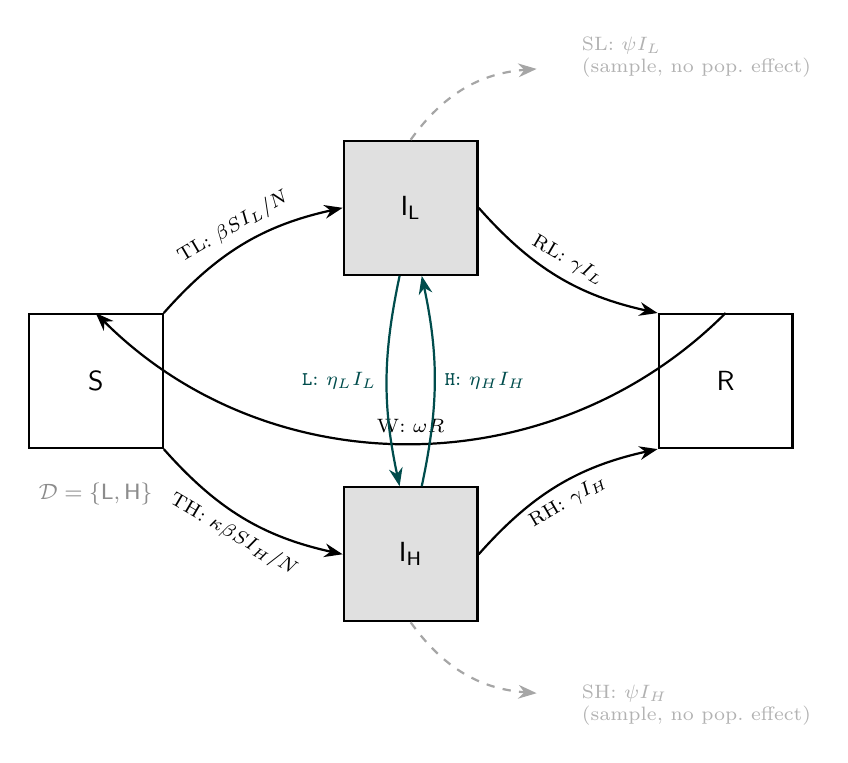
\begin{tikzpicture}[
    >=Stealth,
    compartment/.style={
      rectangle, draw=black, thick, minimum size=1.7cm,
      align=center, font=\bfseries
    },
    deme/.style={fill=black!12},
    flow/.style={->, thick, black},
    mig/.style={->, thick, teal!60!black},
    samp/.style={->, thick, dashed, gray!70},
    lbl/.style={font=\scriptsize}
  ]
  \node[compartment] (S) at (0,0) {$\deme{S}$};
  \node[compartment, deme] (IL) at (4,2.2) {$\deme{I_L}$};
  \node[compartment, deme] (IH) at (4,-2.2) {$\deme{I_H}$};
  \node[compartment] (R) at (8,0) {$\deme{R}$};

  \draw[flow] (S.north east) to[bend left=18]
    node[lbl, above, sloped, pos=0.5] {TL: $\beta S I_L/N$} (IL.west);
  \draw[flow] (S.south east) to[bend right=18]
    node[lbl, below, sloped, pos=0.5] {TH: $\kappa\beta S I_H/N$} (IH.west);

  \draw[flow] (IL.east) to[bend right=18]
    node[lbl, above, sloped, pos=0.5] {RL: $\gamma I_L$} (R.north west);
  \draw[flow] (IH.east) to[bend left=18]
    node[lbl, below, sloped, pos=0.5] {RH: $\gamma I_H$} (R.south west);

  \draw[flow] (R.north) to[bend left=45]
    node[lbl, above, pos=0.5] {W: $\omega R$} (S.north);

  \draw[mig] ([xshift=-4pt]IL.south) to[bend right=12]
    node[lbl, left, pos=0.5, text=teal!60!black] {\code{L}: $\eta_L I_L$}
    ([xshift=-4pt]IH.north);
  \draw[mig] ([xshift=4pt]IH.north) to[bend right=12]
    node[lbl, right, pos=0.5, text=teal!60!black] {\code{H}: $\eta_H I_H$}
    ([xshift=4pt]IL.south);

  \draw[samp] (IL.north) to[bend left=25] ++(1.6,0.9);
  \node[lbl, text=gray!60, align=left, right=0.05cm]
    at ($(IL.north)+(2.0,1.05)$) {SL: $\psi I_L$\\(sample, no pop.\ effect)};

  \draw[samp] (IH.south) to[bend right=25] ++(1.6,-0.9);
  \node[lbl, text=gray!60, align=left, right=0.05cm]
    at ($(IH.south)+(2.0,-1.05)$) {SH: $\psi I_H$\\(sample, no pop.\ effect)};

  \node[font=\footnotesize, below=0.3cm of S, text=black!45]
    {$\Demes = \{\deme{L}, \deme{H}\}$};
\end{tikzpicture}
\caption{The SI2R (superspreading) population model, redrawn from
\code{si2r\_model.qmd} in this report's house style (shaded boxes are the
two demes $\Demes = \{\deme{L}, \deme{H}\}$, matching \code{si2r\_model.qmd}'s
own convention). \code{TL} and \code{TH} are BIRTH marks; \code{L} and
\code{H} (teal) are MIGRATION marks between the two demes; \code{RL}/\code{RH}
are DEATH; \code{W} is NEUTRAL; \code{SL}/\code{SH} (dashed, gray) are
SAMPLE marks with no effect on the population state $x$ --- a sample
changes the genealogy's coloring but not $\Xr_t$, so the dashed stub does
not connect to another compartment.}
\label{fig:si2r-population}
\end{figure}

The reference is \code{si2r\_model.qmd}, a document living in a separate
project directory (\code{efficiency/si2r/}), never used by, cited by, or
consulted during any milestone of the \pkg{PhyloPOMP.jl} compiler.  SI2R was
declared in this package's DSL for the first time in the session that
produced this check.  That document independently hand-derives, from the KLI
paper, an eighteen-line compatibility-indicator/saturation table, closed-form
$\Phi_u$ expressions, and a decay equation
\[
  \lambda = \alpha_{\text{SL}} + \alpha_{\text{SH}}
    + \alpha_{\text{RL}} \indicator{I_L \le \ell_L}
    + \alpha_{\text{RH}} \indicator{I_H \le \ell_H}.
\]
Two of its closed forms are used below: its Eq.~132, giving TL's collapsed
\code{:noop} group as $1 - \binom{\ell_L}{2}\big/\binom{I_L}{2}$, and its
Eq.~135, giving TH's collapsed \code{:noop} group as $1 - \ell_L/I_L$.

The declaration itself (\code{src/examples/mgp\_si2r.jl}) uses the identical
\code{@mgp}/\code{@event} DSL as SEIR and MERS.  The compiler functions run
against it---\code{enumerate\_saturations}, \code{kli\_binomial\_ratio},
\code{full\_transitions}, \code{reduce\_event\_indicator},
\code{total\_decay}---are the generic M02--M04 and M07 code, written for
SEIR and MERS, executed \emph{unmodified}.  There is no SI2R-specific branch
anywhere in the pipeline.

\subsubsection{Mapping to the compiler's output: a structurally new case}

TL reproduces Layer~4's situation on a third model.  Its production
$r = (2,0)$ puts both slots in $\deme{L}$, and at full saturation the
compiler returns
\[
  \varphi_{\text{fork}}^{\text{TL}} = \frac{1}{\binom{I_L}{2}},
\]
the \emph{unordered}-pair Moran/Kingman rate---independent confirmation, on a
model that had no part in Layer~4, of the same identity.

TH is the genuinely new case.  Its production $r = (1,1)$ places one slot in
$\deme{L}$ and one in $\deme{H}$, so its Fork saturation $s = (1,1)$ spans
two \emph{different} demes.  No previously declared model in this codebase
had a reachable two-slot Fork of that shape: MERS's same-deme forks
(TCC, THH) have both slots in one deme, and MERS's cross-deme marks
(THC, TCH) are $r = (1,1)$ but only ever realise a single slot---they never
reach a Fork at all.  The generic code, unprompted, returns
\[
  \varphi_{\text{fork}}^{\text{TH}}
  = \frac{\binom{I_L - \ell_L}{0}}{\binom{I_L}{1}}
    \cdot \frac{\binom{I_H - \ell_H}{0}}{\binom{I_H}{1}}
  = \frac{1}{I_L \, I_H},
\]
an \emph{ordered}-pair rate---one designated slot per deme, no factor of~2
and no binomial---which is exactly the denominator $I_L' I_H'$ appearing in
the QMD's boost equation.  The unordered/ordered distinction is not encoded
anywhere in \code{kli\_binomial\_ratio}; it falls out of the production
vector.  A pipeline that had been pattern-matched to MERS's fork template
would not produce it.

\subsubsection{Numerical verification}

\code{test/kli\_si2r\_test.jl} performs 9276 assertions across eleven
independent sub-testsets, in exact \code{Rational\{Int\}} arithmetic
throughout, with no floating-point tolerance anywhere.  All 9276 pass.  For
the four regular BIRTH and MIGRATION marks, the compiler's $\varphi_u$ was
compared saturation-by-saturation against the QMD's binomial-ratio formulas
over 100 randomly sampled states, under a non-vacuity guard requiring
\code{enumerate\_saturations} to return exactly
$\prod_d (\min(r^u_d, \ell_d) + 1)$ entries---without which a short or empty
enumeration would let the comparison loop assert nothing:

\begin{center}
\renewcommand{\arraystretch}{1.15}
\begin{tabular}{llcc}
\toprule
\textbf{Event mark} & \textbf{$r^u$} &
  \textbf{\# saturations checked} & \textbf{Match} \\
\midrule
TL (low-rate transmission)   & $(2,0)$ & 3/3 per state, 100 states & exact \\
TH (superspreader transmission) & $(1,1)$ & 4/4 per state, 100 states & exact \\
\code{L} (\code{I\_L}\,$\to$\,\code{I\_H}) & $(0,1)$
  & 2/2 per state, 100 states & exact \\
\code{H} (\code{I\_H}\,$\to$\,\code{I\_L}) & $(1,0)$
  & 2/2 per state, 100 states & exact \\
\bottomrule
\end{tabular}
\end{center}

The remaining sub-testsets check: the structural fields ($r^u$, $\Delta_u$,
hazard closures) of all nine marks against the QMD's $\alpha_u$ column; the
\code{full\_transitions} classification
(Identity / InlineSameDeme / CrossDeme / Fork) at a concrete state against
the QMD's stated operator column ($Q_u = 1$ with $y' = y$ / swap / fork);
the Chu--Vandermonde identity; \code{total\_decay} against the decay
equation above, with a non-vacuity guard forcing the $I \le \ell$ boundary
branch actually to fire; TL's fork against $1/\binom{I_L}{2}$; and TH's fork
against $1/(I_L I_H)$.

\begin{remark}[Weighted versus unweighted collapse]
The QMD's claim that its table lines 1\&2 and lines 4\&5 collapse was
checked in two distinct ways, because the obvious reading of it is wrong.
As a \emph{grouping-structure} assertion---does
\code{reduce\_event\_indicator} produce exactly the right number of groups,
with the right transition types in each---it holds directly.  But the raw
group sum $\Phi_u = \sum_s \varphi_u(s)$ of Eq.~(\ref{eq:Phi}) is
\emph{unweighted}, and is a different, generally smaller quantity than the
QMD's closed forms; the two coincide only when the multiplicity is one.
Those forms are recovered with the multiplicity weight, as
$\varphi_{\text{id}} + \binom{\ell_L}{1}\varphi_{\text{inline}}
 = 1 - \binom{\ell_L}{2}\big/\binom{I_L}{2}$ for TL (QMD Eq.~132), whose
inline slot lies in $\deme{L}$, and
$\varphi_{\text{id}} + \binom{\ell_H}{1}\varphi_{\text{inline}}
 = 1 - \ell_L/I_L$ for TH (QMD Eq.~135), whose inline slot lies in
$\deme{H}$ even though the resulting expression is in $\ell_L$ and $I_L$.
This is the same weighting subtlety
found at M09 for MERS's TCC/THH aggregates; it was rediscovered
independently here from the disagreement itself, not assumed from the
earlier finding.  Both readings are asserted separately in the test.
\end{remark}

The comparison against Eqs.~132 and~135 is worth separating from the rest.
Checking the compiler's $\varphi_u$ against the QMD's product-form
binomial-ratio formulas is, in the end, two implementations of one formula
agreeing---useful, but weak evidence.  Eqs.~132 and~135 are algebraically
\emph{simplified} closed forms: the binomials have cancelled, and the
resulting expression no longer resembles the compiler's computation at all.
Agreement there is a substantially stronger signal.

\subsubsection{The falsification experiment}

A test suite that cannot fail proves nothing.  To establish that these 9276
assertions actually discriminate a correct declaration from an incorrect
one, two deliberate bugs were introduced into
\code{src/examples/mgp\_si2r.jl} and the suite re-run.  Each was reverted
immediately afterwards.

\begin{center}
\renewcommand{\arraystretch}{1.3}
\begin{tabular}{p{2.1cm}p{4.0cm}p{2.4cm}p{4.6cm}}
\toprule
\textbf{Mutation} & \textbf{What changed} &
  \textbf{Failed / total} & \textbf{Sub-testsets that caught it} \\
\midrule
1 --- wrong deme in hazard &
  TH's rate $\kappa\beta S I_H/N \to \kappa\beta S I_L/N$
  (copy-paste of TL's $I_L$) &
  2 / 9276 &
  1 of 11: the hazard-versus-$\alpha_u$ testset only \\
2 --- same-deme fork &
  TH's \code{move=fork(I\_H => I\_L, I\_H)} $\to$
  \code{fork(I\_H => I\_H, I\_H)} &
  827 failures $+$ 7 errors / 8885 &
  6 of 11: production-vector structure, $\varphi_u$ values,
  classification, collapse grouping, TH ordered-fork identity,
  QMD simplified closed forms \\
\bottomrule
\end{tabular}
\end{center}

Mutation~1 is the plausible copy-paste slip: the wrong deme's population in
one hazard.  Exactly two assertions failed, both inside the sub-testset that
compares hazard closures against the QMD's $\alpha_u$ column.  The other
9274---every $\varphi_u$, $\Phi_u$, decay, and classification
assertion---passed unchanged, because none of that combinatorial machinery
reads the hazard closure at all.  That is the correct behaviour, not a
missed detection: those checks are hazard-blind by construction, and the one
testset that is not caught it.

Mutation~2 is the structural bug: it makes TH a same-deme fork, which is
precisely what a compiler merely pattern-matching MERS's TCC template onto
TH would emit.  827 assertions failed and 7 errored, out of 8885.  (The
total is lower than 9276 because changing $r^u$ from $(1,1)$ to $(0,2)$ also
changes the size of \code{enumerate\_saturations}'s output, so the
comparison loops run fewer iterations.)  The failures were spread across six
of the eleven independent sub-testsets simultaneously---the raw
production-vector check, the $\varphi_u$ values, the transition
classification, the collapse grouping, the TH-specific ordered-fork
identity, and the QMD's simplified closed forms all disagreed at once.

Two sub-testsets did \emph{not} catch it and passed entirely unchanged: the
Chu--Vandermonde identity (800/800) and the $\Phi_u$-conservation check
(3244/3244).  This is worth stating plainly rather than glossing over, since
it delimits what those checks can establish.  Both are self-consistency
identities: they verify that $\varphi_u$ sums to one over a mark's
saturations, and that each $\Phi_u$ equals the sum of its own group members.
Those statements hold for \emph{any} well-formed declared model, correct or
not, because they test only the compiler's internal bookkeeping and never
compare against an external reference.  They are evidence that the
arithmetic is coherent; they are not evidence that the model is right.  The
remaining three sub-testsets---hazards, decay, and TL's fork---do not depend
on TH's production structure and had no reason to change.

Both mutations were reverted, the model file confirmed byte-identical to its
pre-mutation state, and the full 30542-assertion suite re-run green.

\subsubsection{Why this genuinely helps}

The logical structure differs from Layer~4's and should not be conflated
with it.  Layer~4 is an \emph{external-reference} check: it compares one
compiler output against a textbook result that predates the entire project,
at a single fixed structural pattern.  Layer~5 is a
\emph{generalisation-plus-falsifiability} check, and its reference is
external to this project's \emph{development} rather than to its
\emph{authorship}---the QMD is a separate document, in a separate project,
written without reference to this compiler and never consulted during any
milestone, but it is not literature-external in the way the Moran formula
is.  Layer~5 therefore does not do what Layer~4 does, and does not replace
it.

What it does establish has two parts.  First, generality: the M02--M04 and
M07 functions were written before SI2R existed here, contain no
SI2R-specific branch, and nonetheless reproduce an independently
hand-derived filter---including a production shape, the cross-deme
$r = (1,1)$ fork, that no model available during their development could
exercise.  Fitting-to-the-development-models is ruled out for the slice
checked, because the new case's answer ($1/(I_L I_H)$, ordered) is
numerically different from anything the development models could have
taught the code.

Second, and more decisively, falsifiability.  The worry that motivates
Section~\ref{sec:non-circularity} is a pipeline that echoes back whatever
the DSL declared, so that any declaration ``verifies'' against any
reference.  If that were the situation, Mutation~2 would have sailed through
all 8885 assertions the way Mutation~1 sailed through 9274 of 9276.  It did
not: two-thirds of the independent sub-testsets diverged, in exactly the
places the underlying combinatorics says a changed production vector must
show up.  The suite demonstrably distinguishes a correct SI2R declaration
from an incorrect one.

\subsubsection{Honest scope}

Layer~5 validates the generality of the M02--M04 pipeline
($\varphi_u$ via \code{kli\_binomial\_ratio}, \code{full\_transitions},
\code{reduce\_event\_indicator}) and of M07's \code{total\_decay} across a
genuinely new structural case, against a reference authored outside this
project's development---and it demonstrates by direct falsification that the
test suite discriminates rather than being vacuously true.  It does not
cover:

\begin{itemize}
  \item \textbf{Any compiled filter for SI2R.}  No
    \code{mgp\_si2r\_filter.jl} and no \code{si2r\_naive.jl} exist.  SI2R
    therefore has no Gate-5-style numerical-equivalence check---nothing
    comparable to Layer~3---and none of the driver assembly, proposal-kernel,
    or SMC machinery is exercised for it.

  \item \textbf{The QMD's driver and boost equations as assembled
    expressions.}  Only selected $\varphi_u$ and $\Phi_u$ \emph{values} that
    those equations quote as intermediate quantities were checked, not the
    equations themselves.

  \item \textbf{Parameter regimes beyond the states swept.}  The $\varphi_u$
    comparison covers 100 sampled states with $I_L, I_H \in [2,50]$; the
    classification and collapse checks are made at concrete states.  Nothing
    is claimed for regimes outside those.
\end{itemize}

% Replacement for the existing fig:layers figure (originally in Section 4,
% "Layer 4" subsection, "Honest scope" sub-subsection): adds a fifth,
% topmost layer for the SI2R generalization + falsification evidence.
% This REPLACES the entire existing \begin{figure}[ht] ... \end{figure}
% block that currently produces \label{fig:layers}. Keep the label
% fig:layers unchanged so existing \ref{fig:layers} citations still work.
\begin{figure}[ht]
\centering
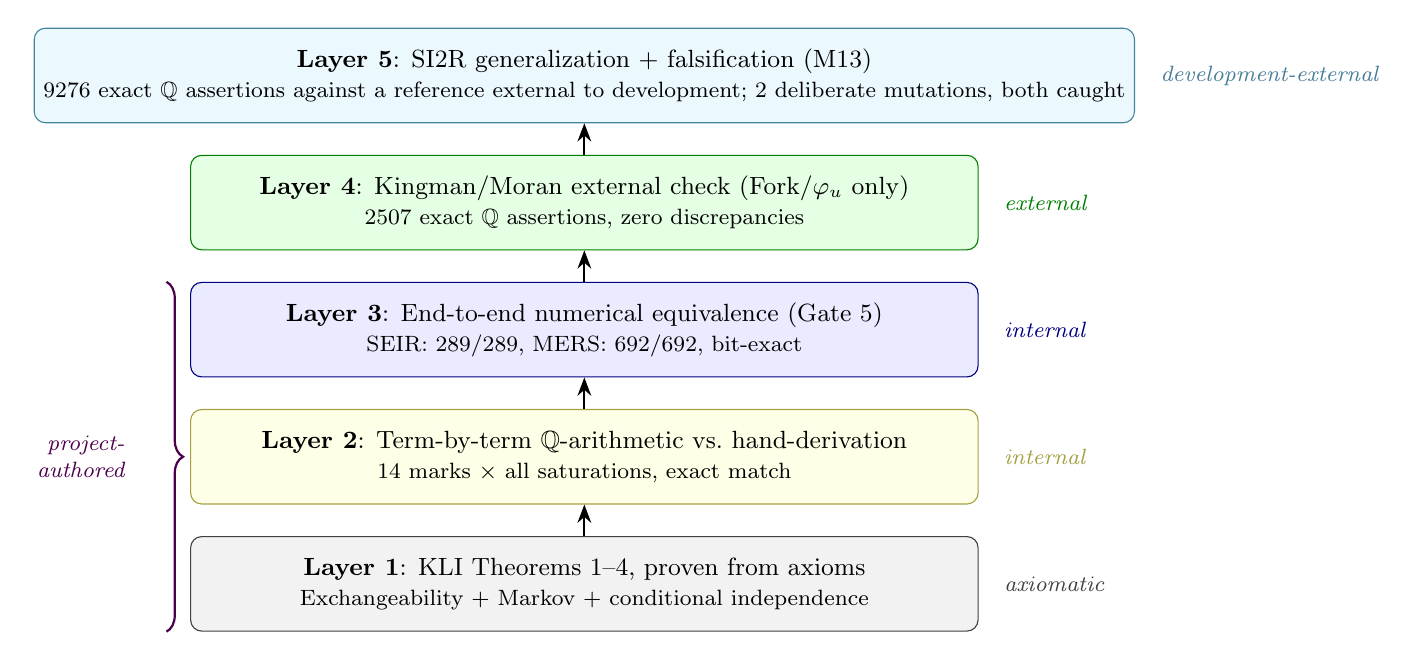
\begin{tikzpicture}[
    >=Stealth,
    layer/.style={
      rectangle, rounded corners=4pt, draw, minimum width=10cm,
      minimum height=1.2cm, align=center, font=\small
    },
    arr/.style={->, thick}
  ]
  \node[layer, fill=cyan!8, draw=cyan!60!black] (l5)
    {\textbf{Layer 5}: SI2R generalization + falsification (M13)\\
     \footnotesize 9276 exact $\mathbb{Q}$ assertions against a reference
     external to development; 2 deliberate mutations, both caught};
  \node[layer, fill=green!10, draw=green!50!black, below=0.4cm of l5] (l4)
    {\textbf{Layer 4}: Kingman/Moran external check
     (Fork/$\varphi_u$ only)\\
     \footnotesize 2507 exact $\mathbb{Q}$ assertions, zero discrepancies};
  \node[layer, fill=blue!8, draw=blue!50!black, below=0.4cm of l4] (l3)
    {\textbf{Layer 3}: End-to-end numerical equivalence (Gate 5)\\
     \footnotesize SEIR: 289/289, MERS: 692/692, bit-exact};
  \node[layer, fill=yellow!10, draw=yellow!60!black, below=0.4cm of l3] (l2)
    {\textbf{Layer 2}: Term-by-term $\mathbb{Q}$-arithmetic vs.\
     hand-derivation\\
     \footnotesize 14 marks $\times$ all saturations, exact match};
  \node[layer, fill=gray!10, draw=gray!50!black, below=0.4cm of l2] (l1)
    {\textbf{Layer 1}: KLI Theorems 1--4, proven from axioms\\
     \footnotesize Exchangeability + Markov + conditional independence};

  \node[font=\footnotesize\itshape, text=cyan!55!black,
        right=0.2cm of l5.east, anchor=west] {development-external};
  \node[font=\footnotesize\itshape, text=green!50!black,
        right=0.2cm of l4.east, anchor=west] {external};
  \node[font=\footnotesize\itshape, text=blue!50!black,
        right=0.2cm of l3.east, anchor=west] {internal};
  \node[font=\footnotesize\itshape, text=yellow!60!black,
        right=0.2cm of l2.east, anchor=west] {internal};
  \node[font=\footnotesize\itshape, text=gray!50!black,
        right=0.2cm of l1.east, anchor=west] {axiomatic};

  \draw[arr] (l1) -- (l2);
  \draw[arr] (l2) -- (l3);
  \draw[arr] (l3) -- (l4);
  \draw[arr] (l4) -- (l5);

  \draw[decorate, decoration={brace,amplitude=6pt,mirror},
        thick, violet!60!black]
    ([xshift=-0.3cm]l1.south west) -- ([xshift=-0.3cm]l3.north west)
    node[midway, left=0.4cm, font=\footnotesize\itshape,
         text=violet!60!black, align=right]
    {project-\\authored};
\end{tikzpicture}
\caption{The five layers of verification, in three distinct categories.
Layer~4 (green) is \emph{literature-external}: it checks against a
textbook combinatorial result (Kingman/Moran) that predates KLI and this
project entirely. Layer~5 (cyan) is \emph{development-external}: it checks
against SI2R (\code{si2r\_model.qmd}), a model specification never
consulted during any milestone of this compiler's development, but not
itself a source independent of this research group the way the Moran
formula is --- a different, weaker-but-still-genuine kind of externality,
strengthened here by a direct falsifiability check (deliberate mutation of
the model declaration) that Layers~1--4 do not perform. Layers~1--3 (grey,
yellow, blue) are internally consistent and mutually reinforcing, but
entirely project-authored, with no external or development-external
reference at all.}
\label{fig:layers}
\end{figure}

\subsection{Additional evidence: property-based testing (M12)}

Beyond the four layers above, M12 added 14{,}489 randomized property
tests across five structural invariants, all passing:

\begin{center}
\renewcommand{\arraystretch}{1.15}
\begin{tabular}{llc}
\toprule
\textbf{Property} & \textbf{Statement} & \textbf{Trials} \\
\midrule
P1 & $\ell_d \le n_d$ preserved by all functions & 400 \\
P2 & $\sum \varphi_u = \sum \Phi_u$ (exact $\mathbb{Q}$) & 500 \\
P3 & $\Phi_u \ge 0$ and $\varphi_u \ge 0$ & 500 \\
P4 & Infeasible inputs $\to$ zero, never error & 400 \\
P5 & Structural invariants on every transition type & 600 \\
\bottomrule
\end{tabular}
\end{center}

\subsection{What remains}

The honest summary, stated plainly rather than inflated:

\begin{itemize}
  \item \textbf{No model has ``exact oracle'' status.}  The strongest
    evidence is ``handwritten implementation comparison'' (Gate~5), for
    SEIR and MERS only.  SI2R has no compiled filter at all, so it has no
    Gate~5 evidence of any kind---its verification stops at the
    M02--M04/M07 compiler stages.

  \item \textbf{The Moran check (Layer~4) is the only external
    check.}  It covers the Fork/$\varphi_u$ slice of the compiler.
    The structured/multi-deme pieces (driver, decay, cross-deme
    migration, the $m$-reduction) remain validated only by internal
    cross-checks.

  \item \textbf{SI2R occupies a middle position.}  It is no longer ``not yet
    independently verified'': its $\varphi_u$, transition classification,
    reduction grouping, and decay were checked term-by-term against a
    reference document authored outside this project's development
    (Layer~5), and the check was shown by falsification to be capable of
    failing.  But SI2R still has no \code{mgp\_si2r\_filter.jl} and no
    \code{si2r\_naive.jl}, so it lacks the Gate-5 compiled-versus-hand-coded
    numerical-equivalence check that SEIR and MERS have.  Closing that gap
    is the obvious next step.

  \item \textbf{BDEI and BDSS} remain ``not yet independently verified'' in
    the original sense: neither model exists in the codebase at all.

  \item The KLI framework's actual novel content---multi-deme
    genealogies, migration, decay/boost corrections---does not reduce
    to a textbook special case, so no external check of comparable rigor
    is available for those pieces.  The Kingman/Moran check is as far
    as the existing literature allows.
\end{itemize}

% ============================================================================
\section*{Acknowledgments}
% ============================================================================

This document was generated from a review of milestones M00--M13 of
the \pkg{PhyloPOMP.jl} compiler project.  The mathematical framework is
due to King, Lin, and Ionides.

\end{document}
